%%%%%%%%%%%%%%%%%%%%%%%%%%%%%%%%%%%%%%%%%
% Journal Article
% LaTeX Template
% Version 1.4 (15/5/16)
%
% This template has been downloaded from:
% http://www.LaTeXTemplates.com
%
% Original author:
% Frits Wenneker (http://www.howtotex.com) with extensive modifications by
% Vel (vel@LaTeXTemplates.com)
%
% License:
% CC BY-NC-SA 3.0 (http://creativecommons.org/licenses/by-nc-sa/3.0/)
%
%%%%%%%%%%%%%%%%%%%%%%%%%%%%%%%%%%%%%%%%%

%----------------------------------------------------------------------------------------
%	PACKAGES AND OTHER DOCUMENT CONFIGURATIONS
%----------------------------------------------------------------------------------------

\documentclass[twoside,twocolumn]{article}

\usepackage{blindtext} % Package to generate dummy text throughout this template 

\usepackage[sc]{mathpazo} % Use the Palatino font
\usepackage[T1]{fontenc} % Use 8-bit encoding that has 256 glyphs
\linespread{1.05} % Line spacing - Palatino needs more space between lines
\usepackage{microtype} % Slightly tweak font spacing for aesthetics

\usepackage[english]{babel} % Language hyphenation and typographical rules

\usepackage[hmarginratio=1:1,top=32mm,columnsep=20pt]{geometry} % Document margins
\usepackage[hang, small,labelfont=bf,up,textfont=it,up]{caption} % Custom captions under/above floats in tables or figures
\usepackage{booktabs} % Horizontal rules in tables

\usepackage{lettrine} % The lettrine is the first enlarged letter at the beginning of the text

\usepackage{enumitem} % Customized lists
\setlist[itemize]{noitemsep} % Make itemize lists more compact

\usepackage{abstract} % Allows abstract customization
\renewcommand{\abstractnamefont}{\normalfont\bfseries} % Set the "Abstract" text to bold
\renewcommand{\abstracttextfont}{\normalfont\small\itshape} % Set the abstract itself to small italic text

\usepackage{titlesec} % Allows customization of titles
\renewcommand\thesection{\Roman{section}} % Roman numerals for the sections
\renewcommand\thesubsection{\roman{subsection}} % roman numerals for subsections
\titleformat{\section}[block]{\large\scshape\centering}{\thesection.}{1em}{} % Change the look of the section titles
\titleformat{\subsection}[block]{\large}{\thesubsection.}{1em}{} % Change the look of the section titles

\usepackage{fancyhdr} % Headers and footers
\pagestyle{fancy} % All pages have headers and footers
\fancyhead{} % Blank out the default header
\fancyfoot{} % Blank out the default footer
\fancyhead[C]{Harvey Hughes $\bullet$ November 2018 $\bullet$ Emmanuel College} % Custom header text
\fancyfoot[RO,LE]{\thepage} % Custom footer text

\usepackage{titling} % Customizing the title section

\usepackage{hyperref} % For hyperlinks in the PDF

\usepackage{graphicx}
\graphicspath{ {images/} }

\newenvironment{reusefigure}[2][htbp]
  {\addtocounter{figure}{-1}%
   \renewcommand{\theHfigure}{dupe-fig}% If you're using hyperref
   \renewcommand{\thefigure}{\ref{#2}}% Figure counter is \ref
   \renewcommand{\addcontentsline}[3]{}% Avoid placing figure in LoF
   \begin{figure}[#1]}
  {\end{figure}}
\usepackage{wrapfig}
\usepackage{amsmath}
\usepackage{xcolor}
%----------------------------------------------------------------------------------------
%	TITLE SECTION
%----------------------------------------------------------------------------------------

\setlength{\droptitle}{-4\baselineskip} % Move the title up

\pretitle{\begin{center}\Huge\bfseries} % Article title formatting
\posttitle{\end{center}} % Article title closing formatting
\title{Random variables and random number generation FTR } % Article title
\author{%
\\
\textsc{Harvey Hughes} \\
\normalsize Emmanuel College \\ % Your institution
\normalsize Lab Date : 17/10/18\\
\normalsize \href{mailto:hh458@cam.ac.uk}{hh458@cam.ac.uk} % Your email address
}
\date{\today} % Leave empty to omit a date
\renewcommand{\maketitlehookd}{%
\begin{abstract}
\noindent
The purpose of this lab was to introduce random variables and how transformations can be used to generate a different probability density. This would be achieved using Matlab to back up theoretical results of random variables. Jacobian, inverse CDF and non linear transformations were investigated. The theory agreed with Matlabs random number generation throughout. The $\alpha$-stable distribution proved to be particularly interesting as it approaches a Gaussian as $\alpha$ goes to two and its pdf can be expressed in the form $cx^{\gamma}$ for large x. The effect of sample size was observed to improve unbiased estimates such as Monte Carlo by $1/\sqrt{N}$ and produce smoother histogram or kernel density plots.
\newline
\end{abstract}
}

%----------------------------------------------------------------------------------------

\begin{document}

% Print the title
\maketitle

%----------------------------------------------------------------------------------------
%	ARTICLE CONTENTS
%----------------------------------------------------------------------------------------

\section{Introduction}
\lettrine[nindent=0em,lines=3]{D}uring the course of the lab various methods and techniques were used to generate distributions of random variables using Matlab. The techniques investigated involved Jacobian transformation, inverse CDF method and $\alpha$-stable distributions. Histogram plots and kernel smoothing functions will be used in order to analyse the pdf of these functions and how sample size effects these estimates. 
\newline
With the objectives being:
\begin{itemize}
\item Introduce the idea of random variables and functions of them\\
\item To use the Jacobian to transform random variables\\
\item To experiment with non uniform random number generation\\
\end{itemize}

%------------------------------------------------


\section{Results and Discussion}
\subsection{1. Uniform and normal random variables}
\begin{figure}[h]
  \centering
    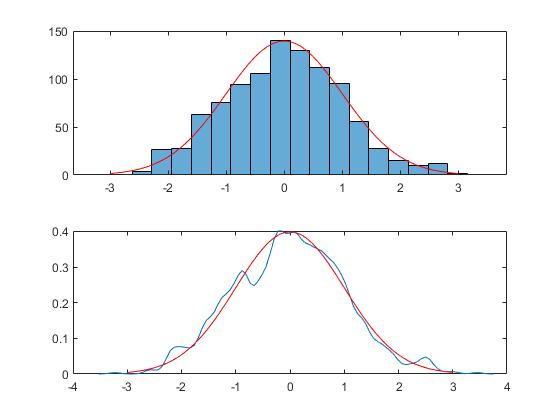
\includegraphics[width=\linewidth]{1normal}
  \caption{Histogram and kernel density plot using a Gaussian kernel $\mathcal{N}(0,1)$ with sample size 1000}
  \label{fig:1normal}
\end{figure}
\begin{figure}[h]
  \centering
    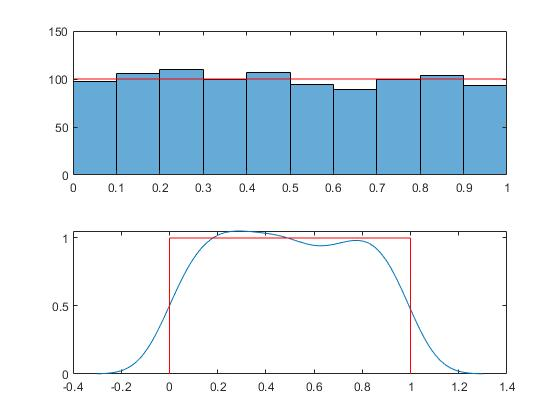
\includegraphics[width=\linewidth]{1uniform}
  \caption{Histogram and kernel density plot using a uniform distribution $\mathcal{U}(0,1)$ with sample size 1000}
  \label{fig:1uniform}
\end{figure}

When a Gaussian kernel is used, as in figure \ref{fig:1normal}, it is clear that a kernel density method to approximate the distribution leads to a more accurate curve. This is due to the smoothing inherent in the kernel density method which removes the jaggedness that is shown in the histogram plot.

The opposite is true for distributions with a large discontinuity in density function such as a uniform distribution pictured in figure \ref{fig:1uniform}. This figure shows the smoothing present with the kernel method either side of the bounds [0,1]. This leads to an incorrect shape of density function. The histogram plot more accurately depicts the distribution due to bin height tending towards the mean as N increases and therefore all bin heights being close to the pdf.
\subsubsection{Multinominal distribution}
When a random vector is drawn from a distribution p(x) and then a histogram plot is generated the multinomial distribution can be calculated. There is a probability ,$p_j$ , that each variable $x^i$ from the random vector lies within the bin limits [a,b]. 
\begin{equation}
\label{multi1}
p_j = \int^{b}_{a}p(x)dx
\end{equation}
All the random variables within the random vector are generated independently and therefore the number of $x^i$'s residing in each bin follows a binomial distribution $\mathcal{B}(p_j,N)$. With the two events being $x^i$ outside or inside the bin limits.  This results in the mean and variable of bin height following equations \ref{eq:1meancal}. The probability of getting $n_i$ variables located in bin $p_i$ follows equation \ref{multi2}. 
\begin{equation}
\label{multi2}
\begin{split}
&p = ^NC_{n_i} p_i^{n_i}(1-p_i)^{N-n_i}\\
&p = \frac{N!}{n_i!(N-n_i)!} p_i^{n_i}(1-p_i)^{N-n_i}\\
&(1-p_i)^{N-n_i} \: is \: the \: probability \: of \: not \: in \: bin \: i\\
&(1-p_i)^{N-n_i} = \Pi_j p_j^{n_j} \frac{N!}{n_j!(N-n_j)!} \:i\neq j \: as \: independant\\
&\Pi_j \frac{N!}{n_j!(N-n_j)!} = \frac{N!}{n_1!n_2!...n_J!}\\
& p = \frac{N!}{n_1!n_2!...n_J!}\Pi_{j=1}^J p_j^{n_i}\\
\end{split}
\end{equation}
\subsubsection{Variation with sample size in uniform variables}
\begin{figure}[h]
  \centering
    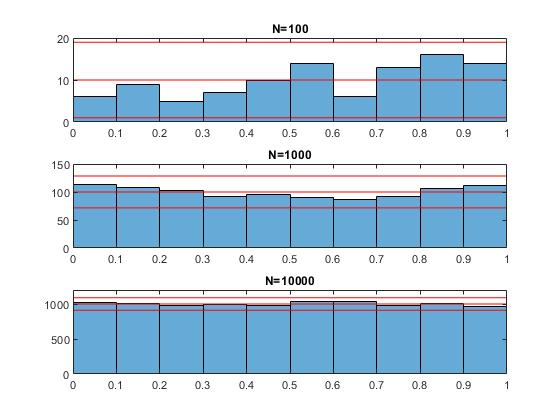
\includegraphics[width=\linewidth]{1means}
  \caption{Histogram plots using a uniform distribution $\mathcal{U}(0,1)$, showing how the theoretical mean and $\pm3\sigma$ of bin height varies with sample size}
  \label{fig:1means}
\end{figure}

\begin{equation}
\label{eq:1meancal}
\begin{split}
&\mu = Np_{j}\\
&\sigma^2=Np_j(1-p_j)\\
\end{split}
\end{equation} 

The theoretical mean and standard deviation of bin height in histogram plots can be calculated using equations \ref{eq:1meancal}. These values have been calculated and plotted in figure \ref{fig:1means} for three different sample sizes from a uniform distribution. $P_j$ is the probability of the distribution being located in one bin, for the plot mentioned $p_j = 0.1$ as 10 bins are present. Table \ref{table:tablemeans} shows the values calculated.
The results observed in figure \ref{fig:1means} show that Matlab accurately generates uniform random variable that agree with the multinomial distribution theory which equation \ref{eq:1meancal} is derived from. As sample size increases the $3\sigma$ lines are relatively closer to the mean height due to standard deviation increasing with $\sqrt{N}$ and mean increasing with N. This agrees with the bin heights becoming far less varied and residing within the $3\sigma$ bounds. These bounds should contain about 99\% of all possible bin heights. 

\begin{table}[h]
\caption{Theoretical mean and standard deviation of bin height for a histogram plot of a uniformly distributed random variable}
\centering
\begin{tabular}{ c | c | c }
Sample Size N & Mean & Standard Deviation \\

\midrule
100 & 10 & 3  \\
1000 & 100 & $3\sqrt{10}$ \\
10000 & 1000 & 30 \\
\end{tabular}
\label{table:tablemeans}
\end{table}
\subsubsection{Variation with sample size in normal variables}
\begin{figure}[h]
  \centering
    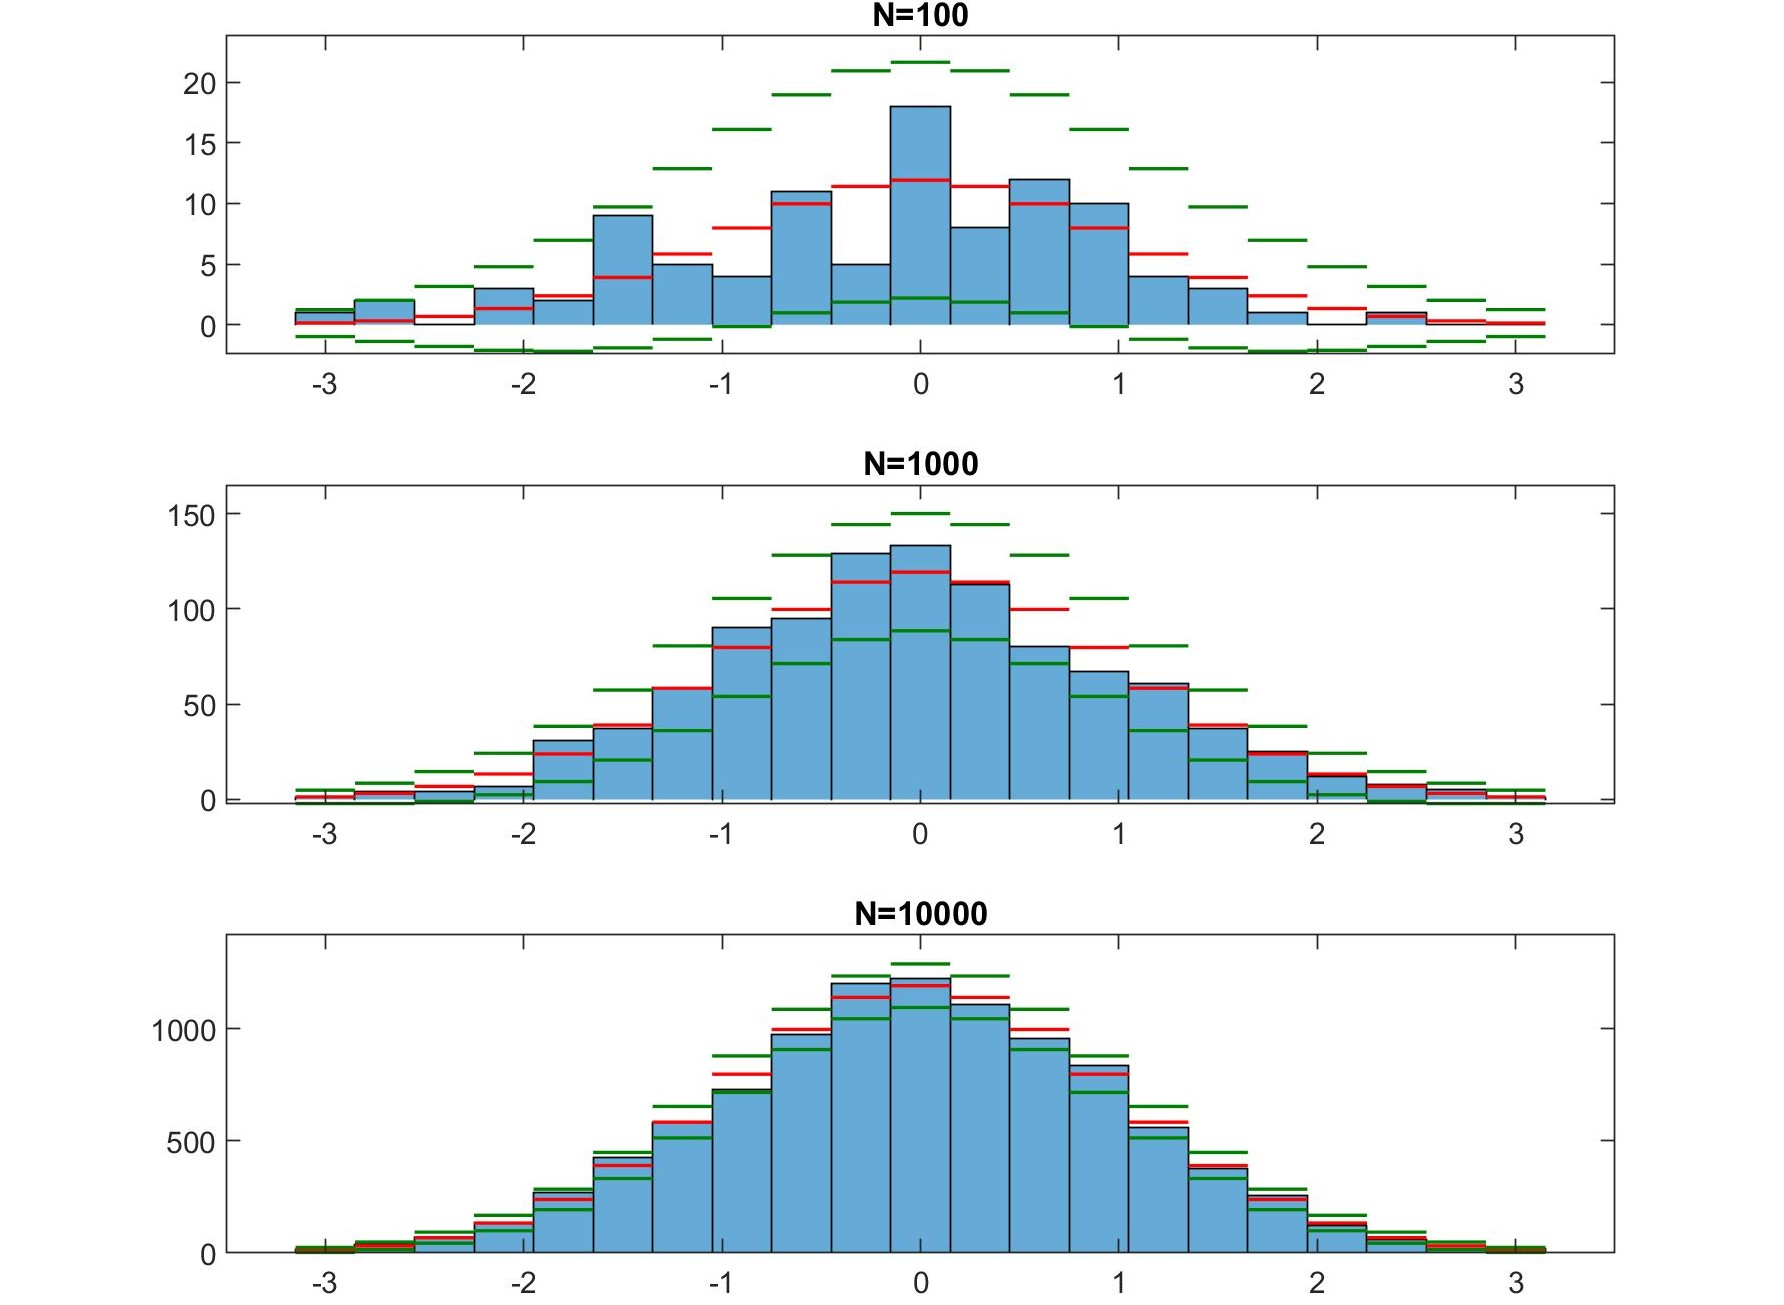
\includegraphics[width=\linewidth]{1fmeans}
  \caption{Histogram plots using a Gaussian distribution $\mathcal{N}(0,1)$, showing how the theoretical mean and $\pm3\sigma$ of bin height varies with sample size}
  \label{fig:1fmeans}
\end{figure}

The multinomial distribution above can also be applied to non uniform random variables. Figure \ref{fig:1fmeans} shows the calculated bin mean heights and variances for a $\mathcal{N}(0,1)$ distribution at various sample sizes. The bin probabilities to be used in equation \ref{eq:1meancal} have been calculated using $p_j=\Phi(upper \:bin \: edge)-\Phi(lower \: bin \: edge)$. Once again it's seen that the relatively proximity of the standard deviation lines to the mean line decreases as N increases. As $p_j$ approaches 0 in the tails of the distribution the $-3\sigma$ lines show a negative density being possible. This is particularly visible for small sample sizes, as variance at small bin probabilities is nearly equal to the mean height (equation \ref{eq:1pivar}) meaning $\mu - 3\sqrt{\mu}$ is likely to be negative. The minima of the -3$\sigma$ line is observed at $\pm$1.8 when N=100, this is at an intermediate bin due to the rate at which the Gaussian distribution decreases here (which is linked to the mean bin height) compared to how the variance decreases. When bin probability is one then we only have one histogram bin with height N and no variance which is to be expected.

\begin{equation}
\label{eq:1pivar}
\begin{split}
&\mu = Np_{j}\\
&\sigma^2=Np_j(1-p_j) = Np_j-Np_j^2\\
&When \: p_j \: small \: \sigma^2\approx Np_j=\mu\\
&This \: is \: more \: true \: when \: N \: is \: also \: small\\ 
\end{split}
\end{equation} 

\subsubsection{Matlab code}%----------------------------
For the Matlab code see section 1.0 and 1.1 of the appendix. With figures \ref{fig:1normal} to \ref{fig:1means} generated in section 1.0 and figure \ref{fig:1fmeans} in 1.1.
%---------------------------------------------------
\subsection{2. Function of random variables}
\subsubsection{Transformation Y=aX+b}
\begin{figure}[h]
  \centering
    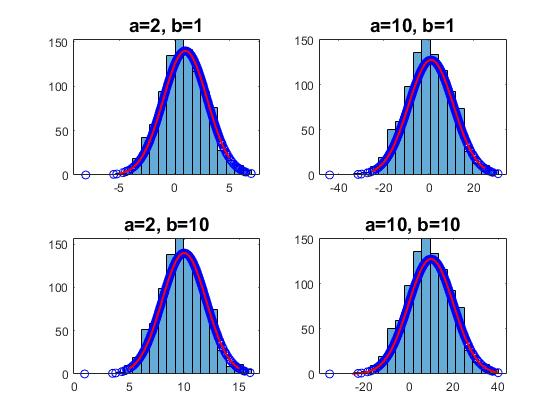
\includegraphics[width=\linewidth]{2linear}
  \caption{Histogram plot of transforming a Gaussian kernel $\mathcal{N}(0,1)$ by $f(x)=ax+b$ with sample size 1000}
  \label{fig:2linear}
\end{figure}

Starting with the distribution $X\sim\mathcal{N}(0,1)$ and performing the transformation Y=aX+b leads to the distribution plotted in figure \ref{fig:2linear}. This is the distribution $Y\sim\mathcal{N}(a\mu+b,\sigma^2a^2)=\mathcal{N}(b,a^2)$. The derivation for this can be seen in equations \ref{eq:2linearder}. Figure \ref{fig:2linear} shows the histogram data for a sample of 1000 variables in addition to each variable being transformed individually using the Jacobian to form the dotted distribution shown. 

\begin{equation}
\label{eq:2linearder}
\begin{split}
&f(X)=aX+b\\
&J=|f'(x)|=|a|\\
&p(y) = \sum_{1}^{1} \frac{p(x)}{J} = \frac{p(\frac{y-b}{a})}{|a|} \\
&p(y)=\frac{1}{a\sigma\sqrt{2\pi}}exp(-\frac{1}{2}[\frac{y-b-a\mu}{a\sigma}]^2)\\
&Y\sim\mathcal{N}(a\mu+b,a^2\sigma^2)\\
\end{split}
\end{equation} 

\subsubsection{Transformation $Y=X^2$}

\begin{figure}[h]
  \centering
    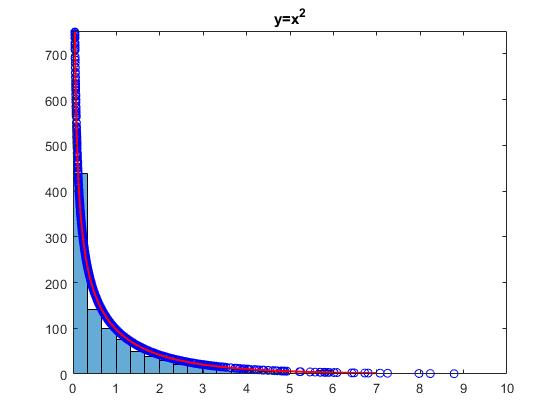
\includegraphics[width=\linewidth]{2quadratic}
  \caption{Histogram plot of transforming a Gaussian kernel $\mathcal{N}(0,1)$ by $f(x)=x^2$ with sample size 1000}
  \label{fig:2quadratic}
\end{figure}

The transformation $Y=X^2$ was applied to another Gaussian distribution following $X\sim\mathcal{N}(0,1)$. Figure \ref{fig:2quadratic} shows the result of this. The distribution $p(y)=\frac{1}{\sqrt{y2\pi}}exp(-\frac{1}{2}y)$ is overlain. This distribution was calculated using the same Jacobian method and is shown in equations \ref{eq:2quadraticder}. As $Y=X^2$ is not a 1:1 function the derivation required summing over all possible y values for a given x.


\begin{equation}
\label{eq:2quadraticder}
\begin{split}
&f(X)=X^2\\
&J=|f'(x)|=2|X|=2\sqrt{y}\\
&p(y) = \sum_{1}^{2} \frac{p(x)}{J} = \frac{p(+\sqrt{y})+p(-\sqrt{y})}{2\sqrt{y}}\\
&p(y)=\frac{p(\sqrt{y}))}{\sqrt{y}}\: by\:symmetry\\
&p(y)=\frac{1}{\sigma\sqrt{y2\pi}}exp(-\frac{1}{2}[\frac{\sqrt{y}-\mu}{\sigma}]^2)\\
&\:\sigma=1,\:\mu=0\\ 
\end{split}
\end{equation} 

\subsubsection{Sine transformations}
\begin{figure}[h]
  \centering
    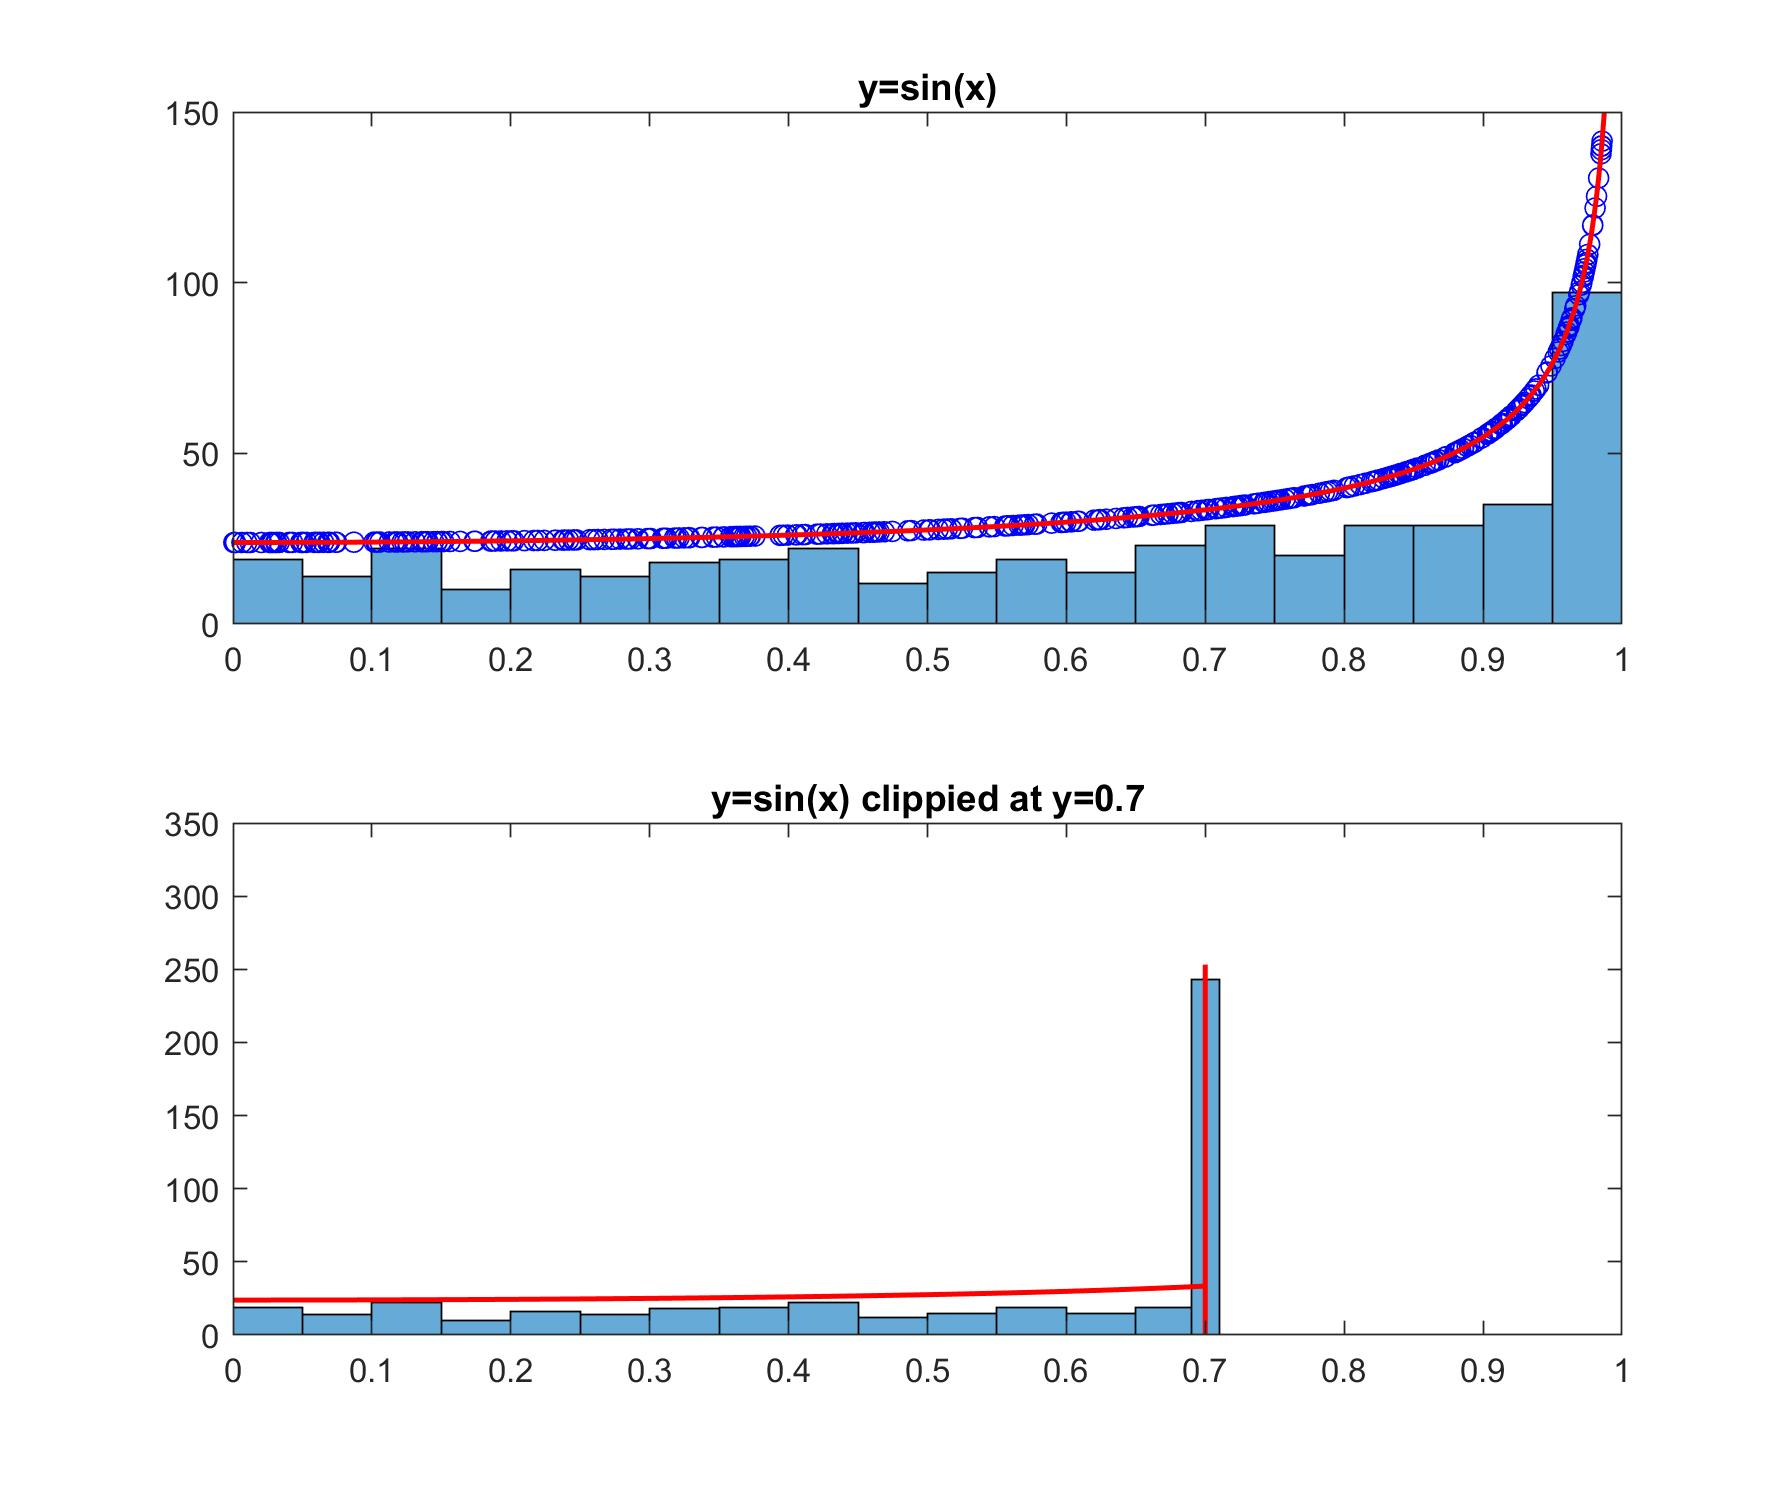
\includegraphics[width=\linewidth]{2sine}
  \caption{Histogram plot of transforming a uniform kernel $\mathcal{N}(0,2\pi)$ by $f_1(x)=sin(x)$ and $f_2(x)=min[sin(x),x]$ with sample size 1000}
  \label{fig:2sine}
\end{figure}

The transformation $Y=sin(X)$ was applied to a uniform distribution $\mathcal{U}(0,2\pi)$. Figure \ref{fig:2sine} shows the end result. A distribution of $p(y)=\frac{1}{2\pi|cos(sin^{-1}(y))|}$ was generated. This is shown overlaid on the histogram plot and each random sample transformed individually. The derivation for this using the Jacobian can be seen in equations \ref{eq:2qsineder}.

\begin{equation}
\label{eq:2qsineder}
\begin{split}
&f(X)=Sin(X)\\
&y=Sin^{-1}(x) \: this \: is \: simplified \: from \: the\\
&2:1 \: case\: due \:to\: p(x)\: being\: uniformly\\
&  distributed \: therefore\: each\: inversion\: case  \\
&will \: contribute \: half\: towards\: p(y)\\ 
&J \: is \: also \: periodic \: so \: each \: half \\
&is \: the \: same\\
&J=|f'(x)|=|cos(x)|=|cos(sin^{-1}(y))|\\
&p(y) = \sum_{1}^{1} \frac{p(x)}{J} = \frac{p(sin^{-1}(y))}{|cos(sin^{-1}(y))|}\\
&p(y)=\frac{1/2\pi}{|Cos(sin^{-1}(y))|}\\
&p(y)=\frac{1}{2\pi|Cos(sin^{-1}(y))|}\\ 
\end{split}
\end{equation} 

\begin{figure}[h]
  \centering
    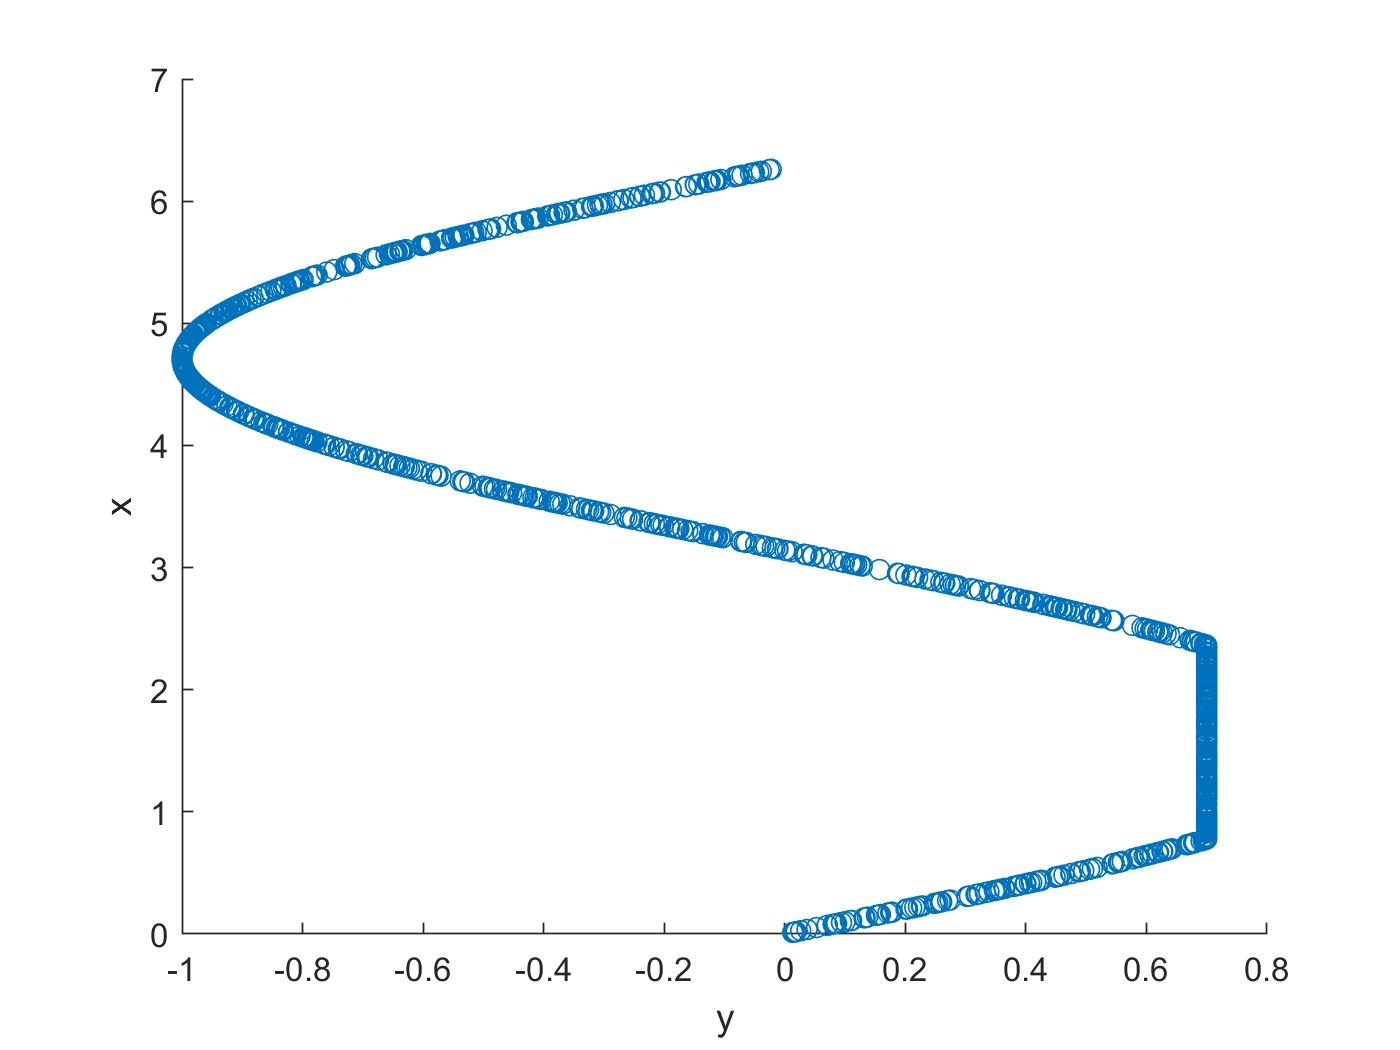
\includegraphics[width=\linewidth]{2clipped}
  \caption{Plot of the transformation $f(x)=min[sin(x),x]$, with  }
  \label{fig:2sine}
\end{figure}

A clipped version of this transformation was considered next $f(x)=min[sin(x),x]$. This can be also be seen in figure \ref{fig:2sine}. p(y) follows the same distribution as before $p(y)=\frac{1}{2\pi|cos(sin^{-1}(y))|}$ for 0<y<0.7, with a spike of magnitude $\frac{\pi-2sin^{-1}(0.7)}{2\pi}$ at y=0.7. The derivation for this extra part are shown in equations \ref{eq:2qsineder2}, for 0<y<0.7 the derivation in equations \ref{eq:2qsineder} still holds. The magnitude of this spike should equal the size of interval in x being truncated, multiplied by the constant p(x) in order for $\int p(y) dy =1 $. This agrees with the derivation shown.

\begin{equation}
\label{eq:2qsineder2}
\begin{split}
&f(x)=min[sin(x),x]\\
&sin^{-1}(0.7) < x < \pi-sin^{-1}(0.7)\\
&y=0.7\\
&\frac{1}{J}=|\frac{dx}{dy}|=2[\frac{\pi}{2}-sin^{-1}(0.7)]\delta(y-0.7)\\
&p(y) = \int^{y=0.7}_{y=0.7} p(x)\frac{1}{J} dy \\
&p(y)=\frac{(\pi-2sin^{-1}(0.7))}{2\pi}\delta(y-0.7)\\
\end{split}
\end{equation}


\subsubsection{Matlab code} %-------------------------
The Matlab code for the transformation Y=aX+b can be seen in section 2.0 of the appendix, the transformation $Y=X^2$ is shown in section 2.1. Section 2.2 includes the code for generating the sine two transformation.
%---------------------------------------------------
\subsection{3. Inverse CDF method}
\subsubsection{Generating an exponential distribution}
\begin{figure}[h]
  \centering
    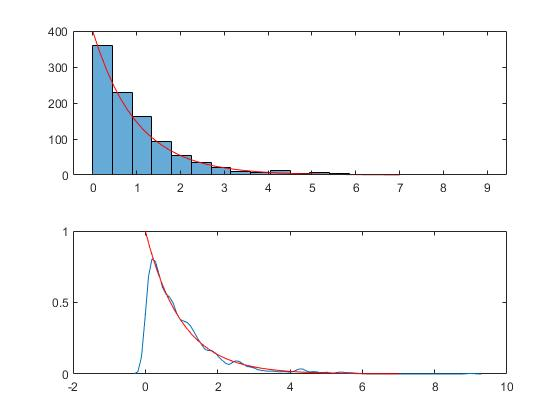
\includegraphics[width=\linewidth]{3exp}
  \caption{Histogram and kernel density plot of an exponential distribution generated using the inverse CDF method on a uniform kernel $\mathcal{U}(0,1)$ with sample size 1000}
  \label{fig:3exp}
\end{figure}
 
\begin{equation}
\label{eq:3cdf}
\begin{split}
&CDF = \int_0^yp(y)dy=\int_0^ye^{-y}\\
&CDF = 1- e^{-y} = F(y)\\
&F^{-1}(y) = -ln(1-y)\\
\end{split}
\end{equation} 



The cumulative distribution function (CDF) for an exponential distribution p(y) = $e^{-y}$ is calculated in equations \ref{eq:3cdf}. Though the use of the inverse CDF and equation \ref{eq:3gen} an exponentially distributed random variable can be generated using a uniform kernel $\mathcal{U}(0,1)$. This generated distribution is shown in figure \ref{fig:3exp} with p(y) overlain. The curves match up with great accuracy especially the kernel density plot. This shows the validity of this method in generating different random variable densities.    

\begin{equation}
\label{eq:3gen}
y^{i} = F^{-1}(x^i)
\end{equation}

\subsubsection{Monte Carlo estimation}

\begin{figure}[h]
  \centering
    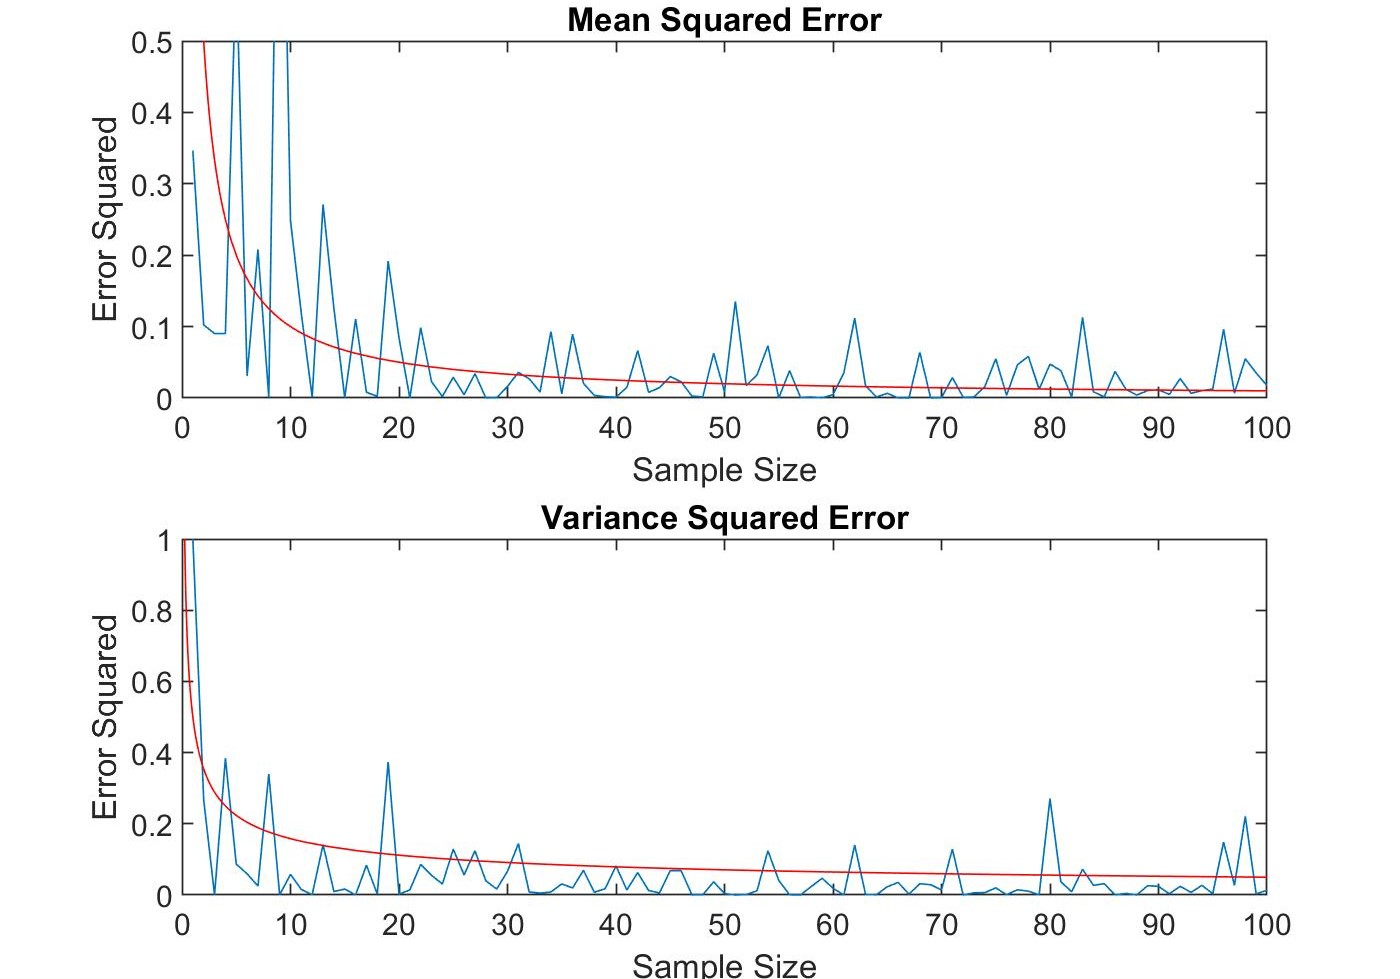
\includegraphics[width=\linewidth]{3monte}
  \caption{Error squared of the Monte Carlo estimator on the exponential distribution, for sample sizes up to 100. Mean squared error is stretched by 5 to more closely match the line.}
  \label{fig:3monteg}
\end{figure}
\begin{figure}[h]
  \centering
    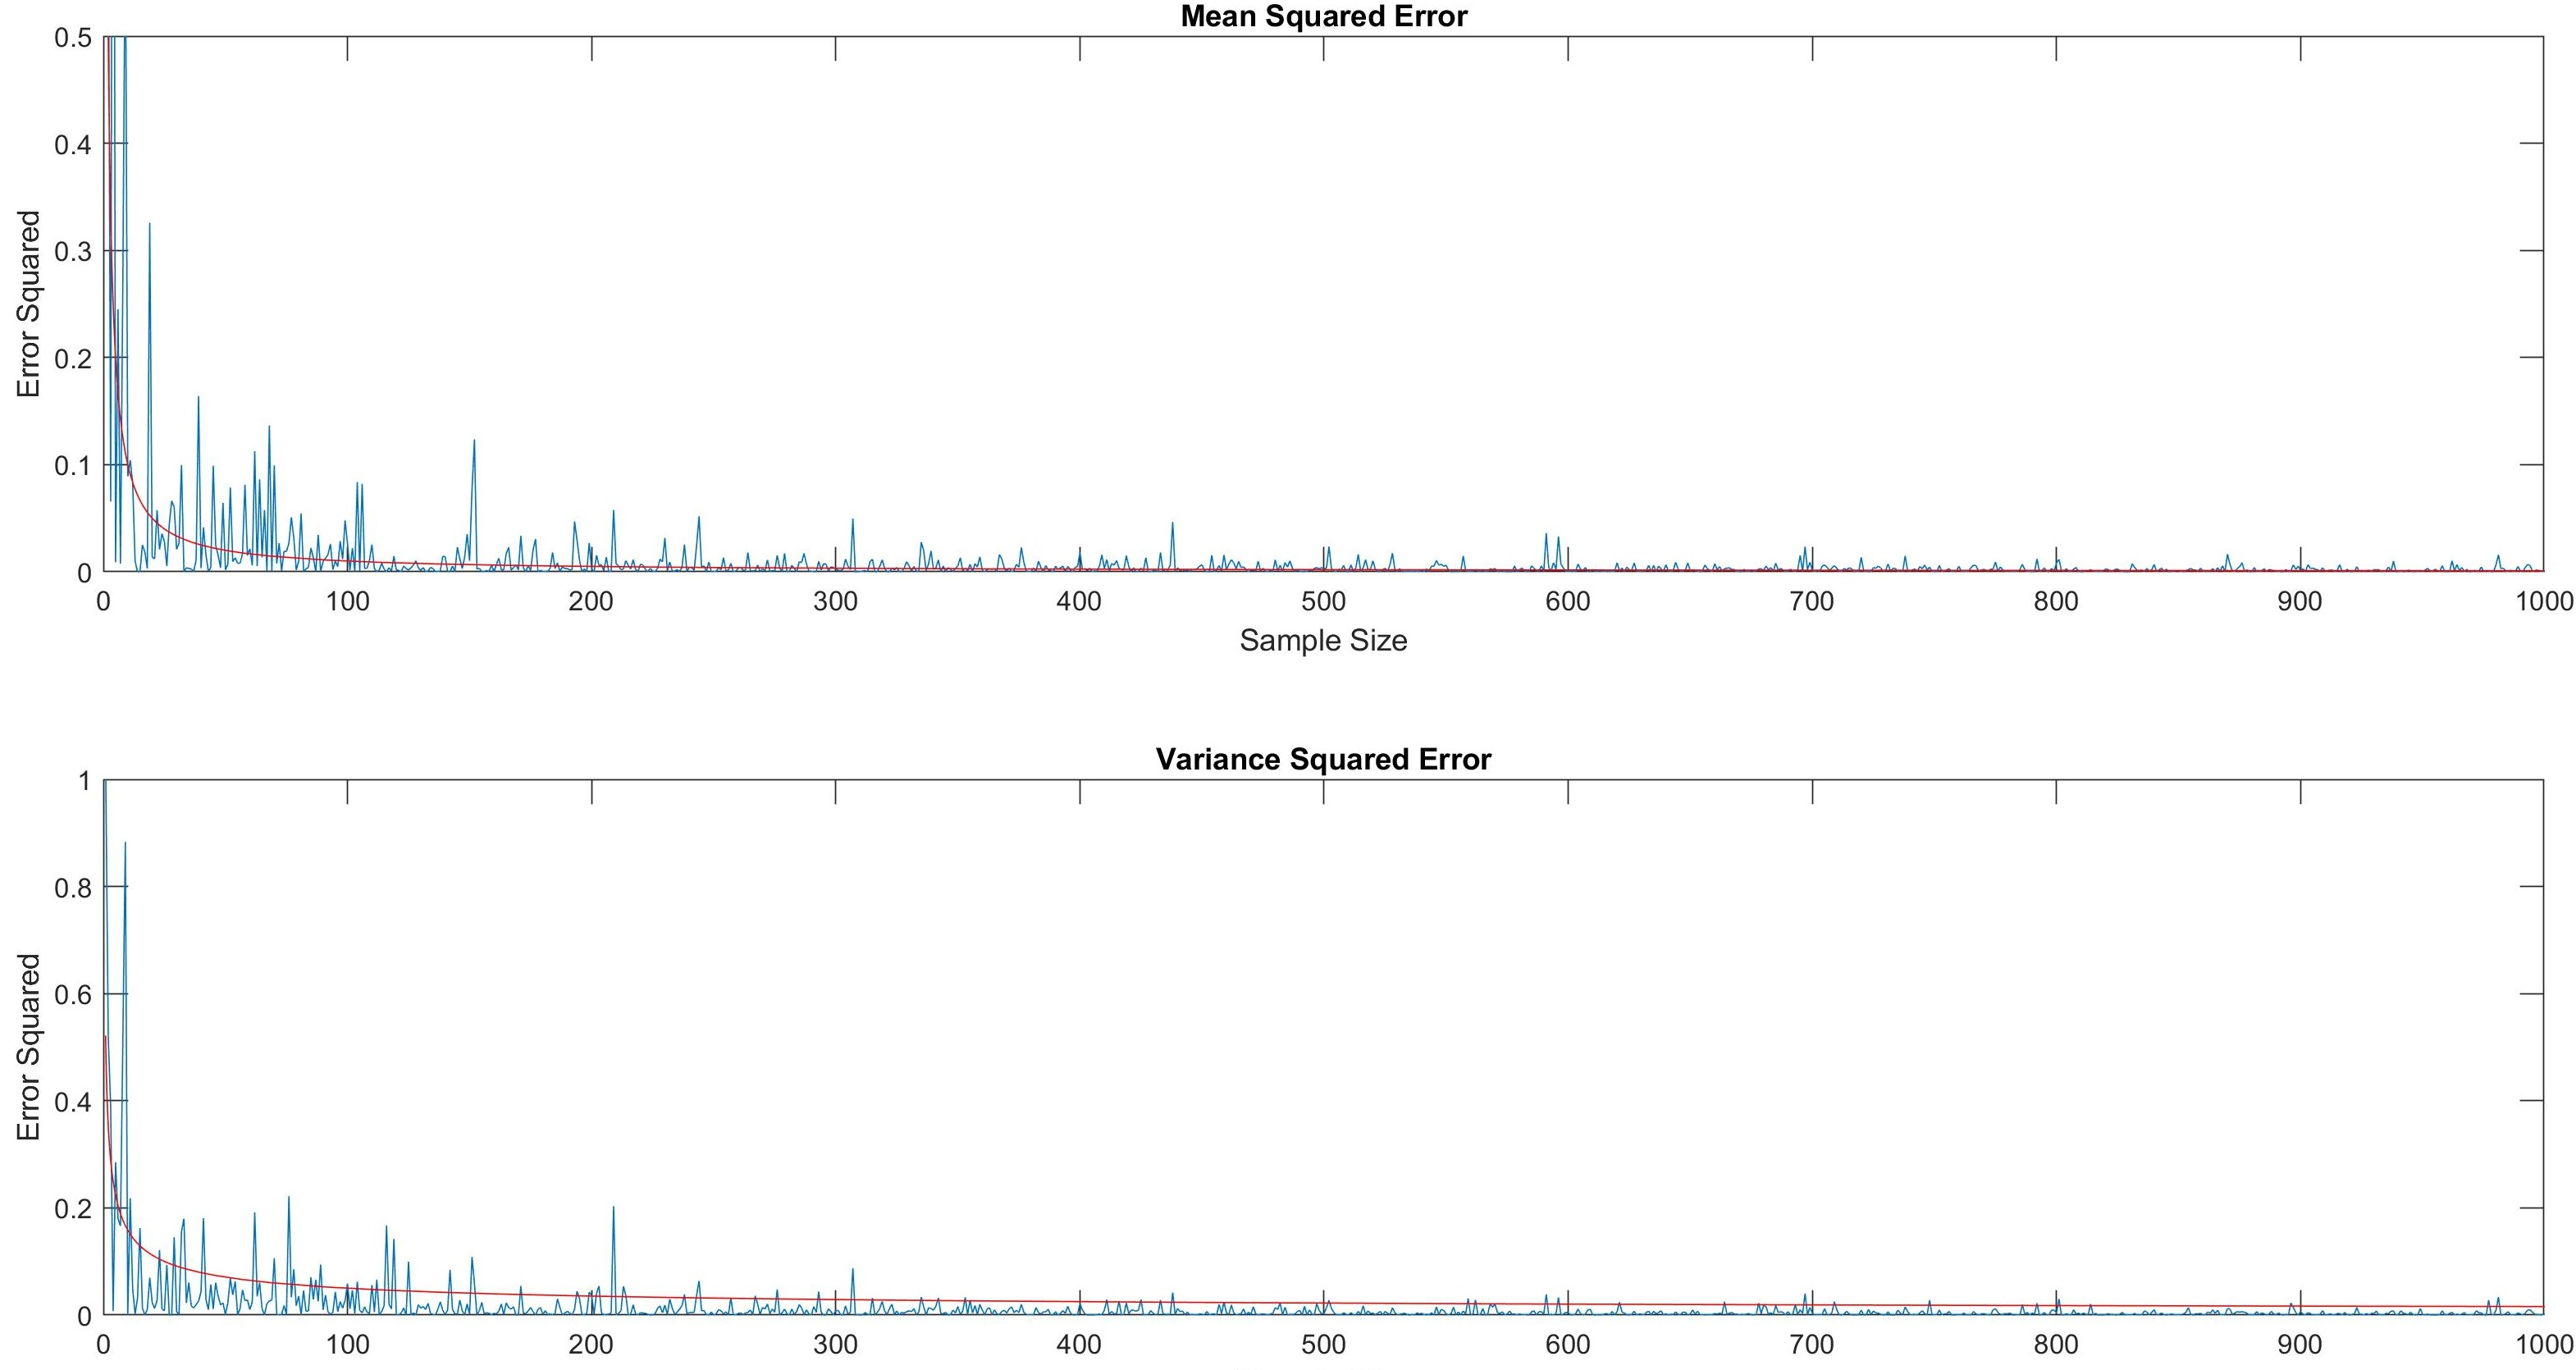
\includegraphics[width=\linewidth]{3ftr2}
  \caption{Error squared of the Monte Carlo estimator on the exponential distribution, for sample sizes up to 1000}
  \label{fig:3m2}
\end{figure}
\begin{figure*}[h]
  \centering
    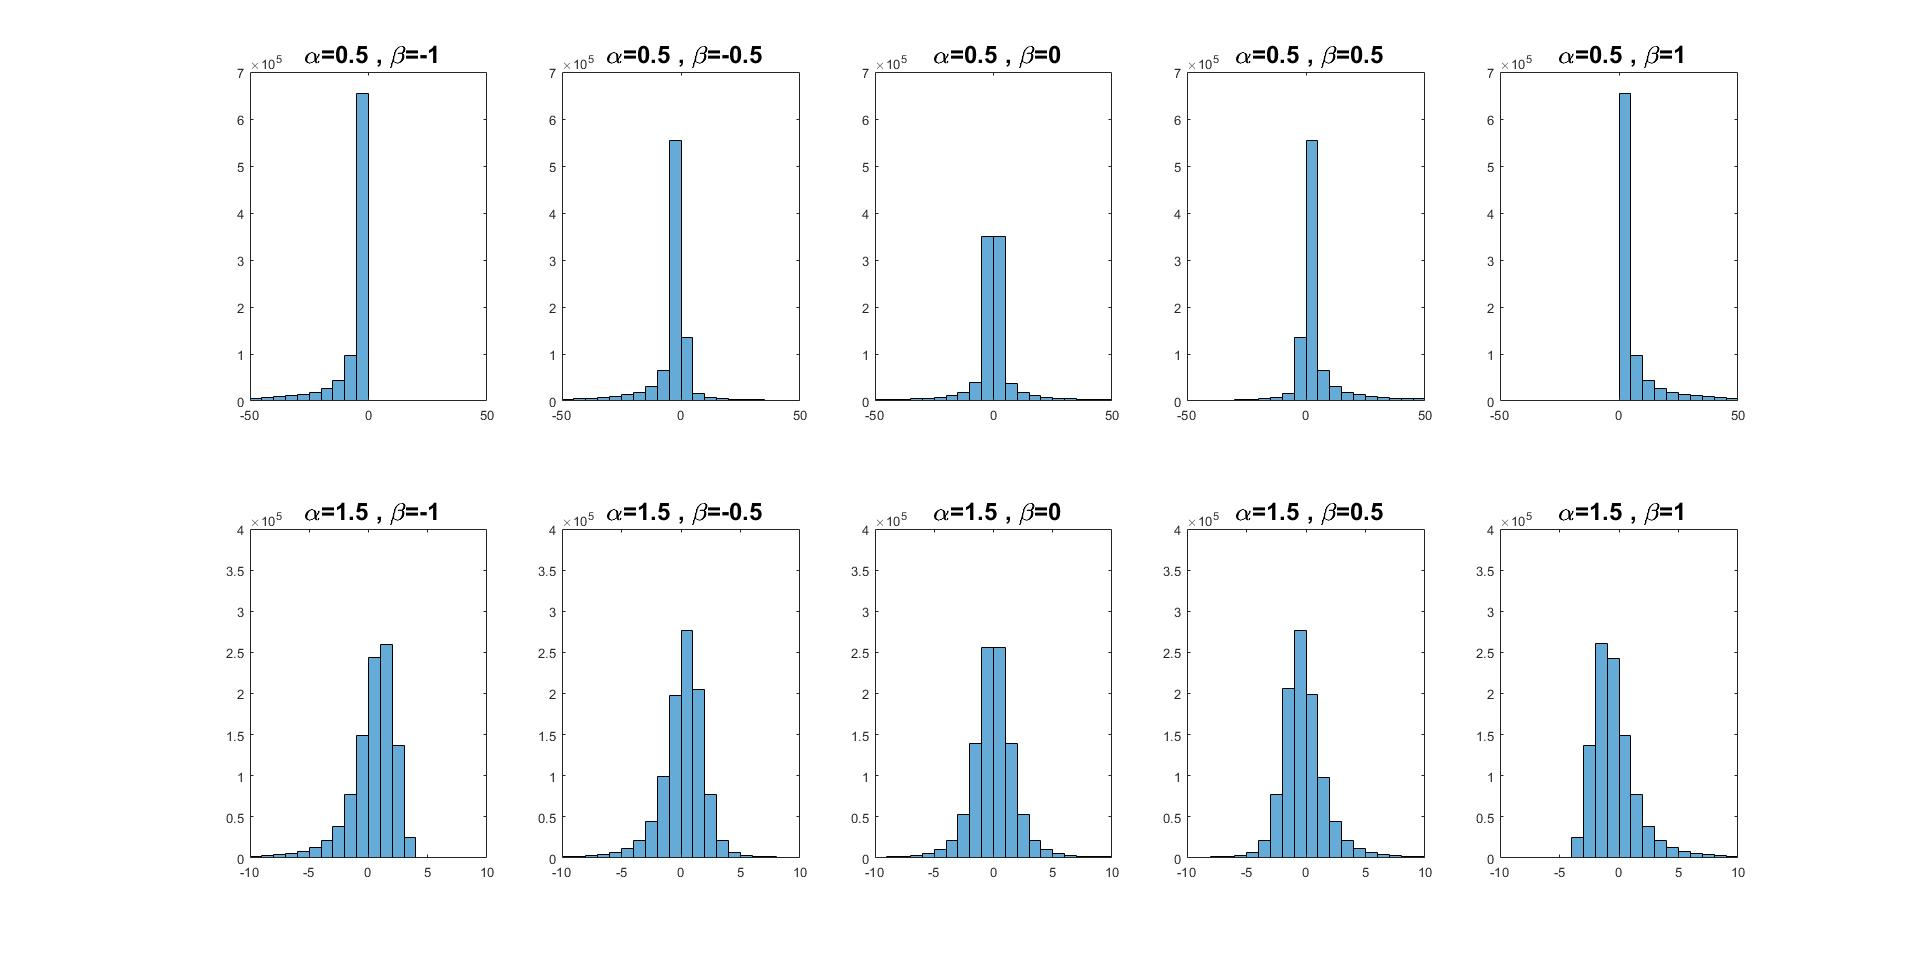
\includegraphics[width=\textwidth ]{4dist}
  \caption{Histogram plots of distribution X in equation \ref{eq:4equ} using various values for constants a and b, all from the same kernels $\mathcal{U}(-\frac{\pi}{2},\frac{\pi}{2})$ and $\mathcal{E}(1)$ with sample size 1000.}
  \label{fig:4dist}
\end{figure*}
The Monte Carlo estimate for mean and variance (equation \ref{eq:3monte}) was used to estimate the these parameters for the generated exponential distribution. This estimate regularly produces means and variances within 0.05 of the theoretical value when sample size is 1000. This is an unbiased estimator as when sample size increases the estimator tends closer to the true value $\mu$ therefore $\mathbb{E}(\hat{\mu})=\mu$. With sample size 100 million the estimator is within 0.001 of the true value.

\begin{equation}
\label{eq:3monte}
\mu = \mathbb{E}[Y]=\int^{\infty}_{y=0}yp(y)dy \approx \frac{1}{N}\sum\limits^N_{i=1}y^i = \hat{\mu}
\end{equation} 

The convergence of this estimator towards the true mean follows a $1/\sqrt{N}$ rate. This can be seen in figures \ref{fig:3monteg} and \ref{fig:3m2} where the squared error is plotted as sample size increases. This error squared follows a 1/N line. The estimators in the graph have been generated from different random sequences for each sample size and repeated three times for each size. The sequences were generated using the exponential distribution previously discussed. From figure \ref{fig:3m2} the error can be seen to be very small at large sample sizes, with the occasional spike due to the variance of this estimator.

\subsubsection{Matlab code} %-------------------------
The Matlab code for the inverse CDF method can be seen in section 3.0 of the appendix. The code for the Monte Carlo estimator is shown in section 3.1.

%---------------------------------------------------
\subsection{4. Simulation from a 'difficult' density}




By using the non linear transformation listed in equations \ref{eq:4equ} and various values for $\alpha$ and $\beta$ the graphs in figure \ref{fig:4dist} can be produced. These graphs indicate that $\alpha$ controls the tail thinness and sharpness of central peak, with a low alpha resulting in a thin tail and sharp centre. A low $\alpha$ such as 0.5 results in a very sharp density peak at 0. $\beta$ appears to affect the skew of the distribution. A negative $\beta$ results in negative skew and vice versa. 


\begin{equation}
\label{eq:4equ}
\begin{split}
&\alpha \in (0,2) \: \beta \in [-1,1]\\
&b=\frac{1}{\alpha}tan^{-1}(\beta tan(\frac{\pi\alpha}{2}))\\
&s=(1+\beta^2tan^2(\frac{\pi\alpha}{2}))^{\frac{1}{2\alpha}}\\
&U\sim\mathcal{U}(-\frac{\pi}{2},\frac{\pi}{2})\:V\sim\mathcal{E}(1)\\
& X=s\frac{sin(\alpha(U+b))}{(cosU)^{1/\alpha}}%(\frac{cos(U-\alpha(U+b))}{V})^{\frac{1-\alpha}{\alpha}}\\
\end{split}
\end{equation}
\subsubsection{Tail behaviour }
The tail probabilities of this distribution can be calculated by counting how many random variables lie outside a certain value. This was conducted with the distribution with $\beta = 0 $ and $ \alpha =0.5 , 1.5$, the results are shown in table \ref{table:tail}. The Gaussian distribution's tail is far smaller and reaches less then 1\% at t=3 however the generated distributions both still have significant probabilities at this t value. The tail is thinner when alpha is 1.5 compared to 0.5 as previously noticed.  

\begin{table}[h]
\caption{Tail probabilities for the distribution with $\beta = 0 $ and $\alpha =0.5 , 1.5$ for four locations(t)}
\centering
\begin{tabular}{ c | c | c | c | c}
Alpha & t=0 & 1 & 3 & 6 \\

\midrule
0.5 & 1 & 0.5467 & 0.3749 & 0.2850 \\
1.5 & 1 & 0.4896 & 0.1053 & 0.0304\\
Gaussian & 1 & 0.3173&0.0027 &0.0000 \\
\end{tabular}
\label{table:tail}
\end{table}

\begin{figure*}[h]
  \centering
    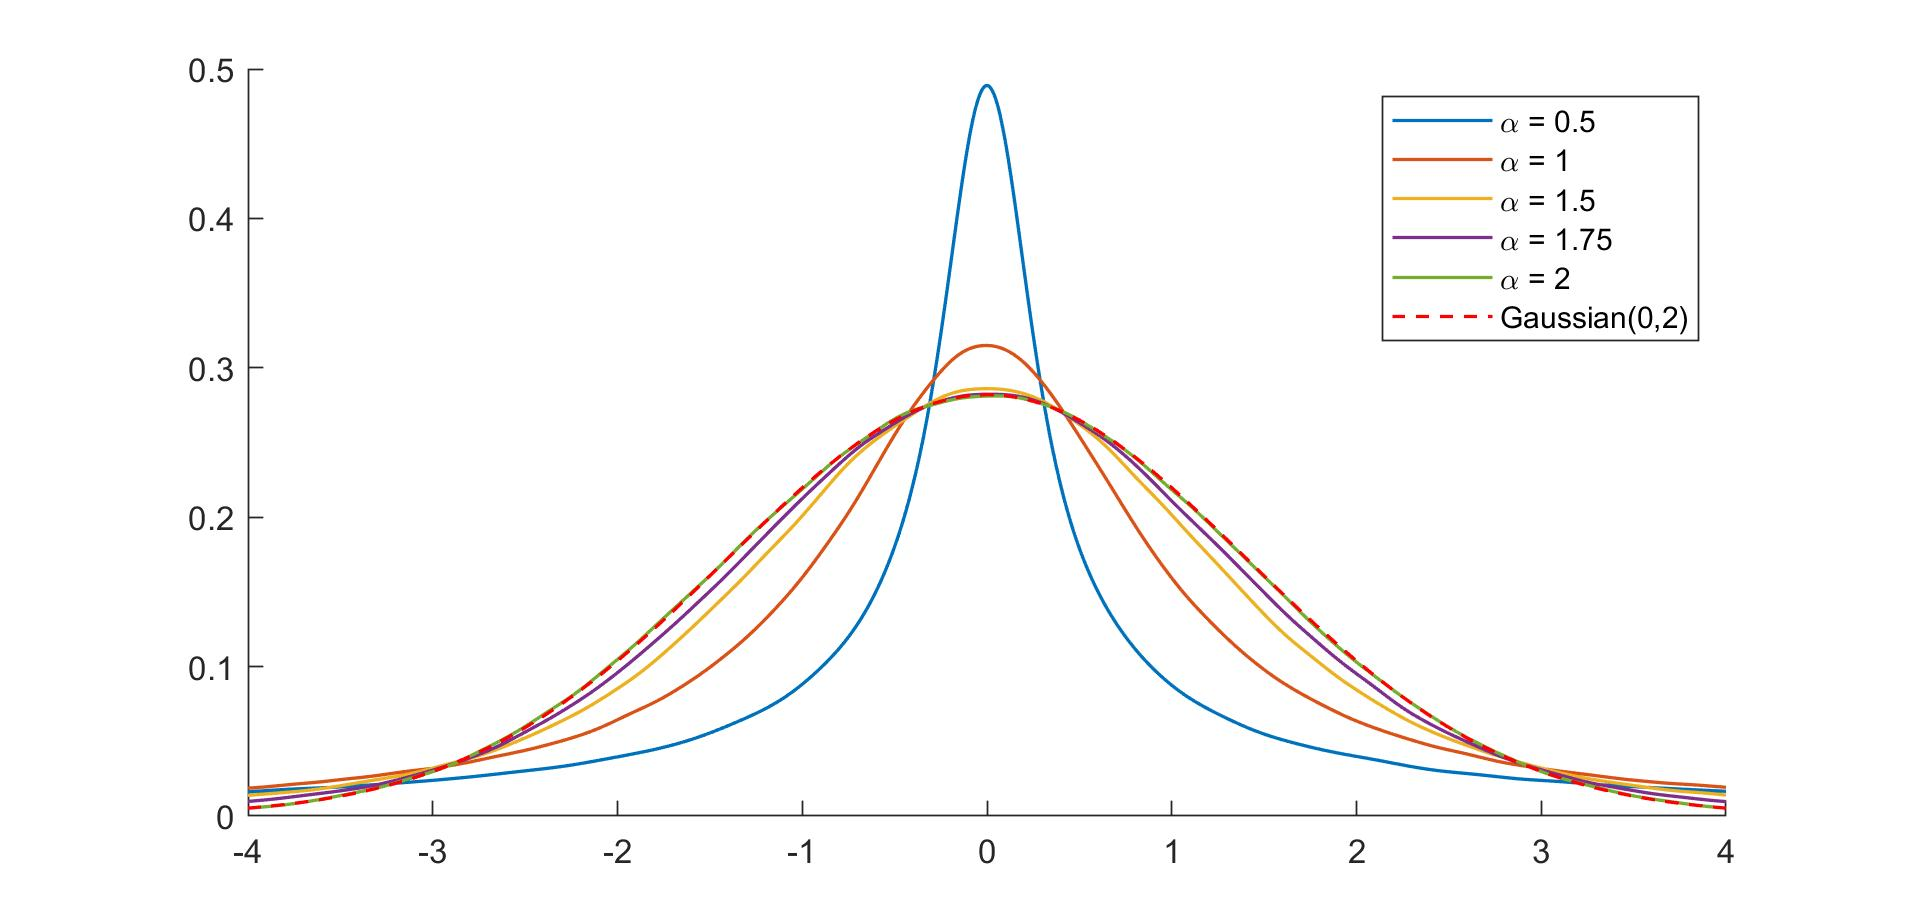
\includegraphics[width=\textwidth]{4ftr3}
  \caption{Pdf of the distribution for various $\alpha$ values.}
  \label{fig:4ftr3}
\end{figure*}
\begin{figure}[h]
  \centering
    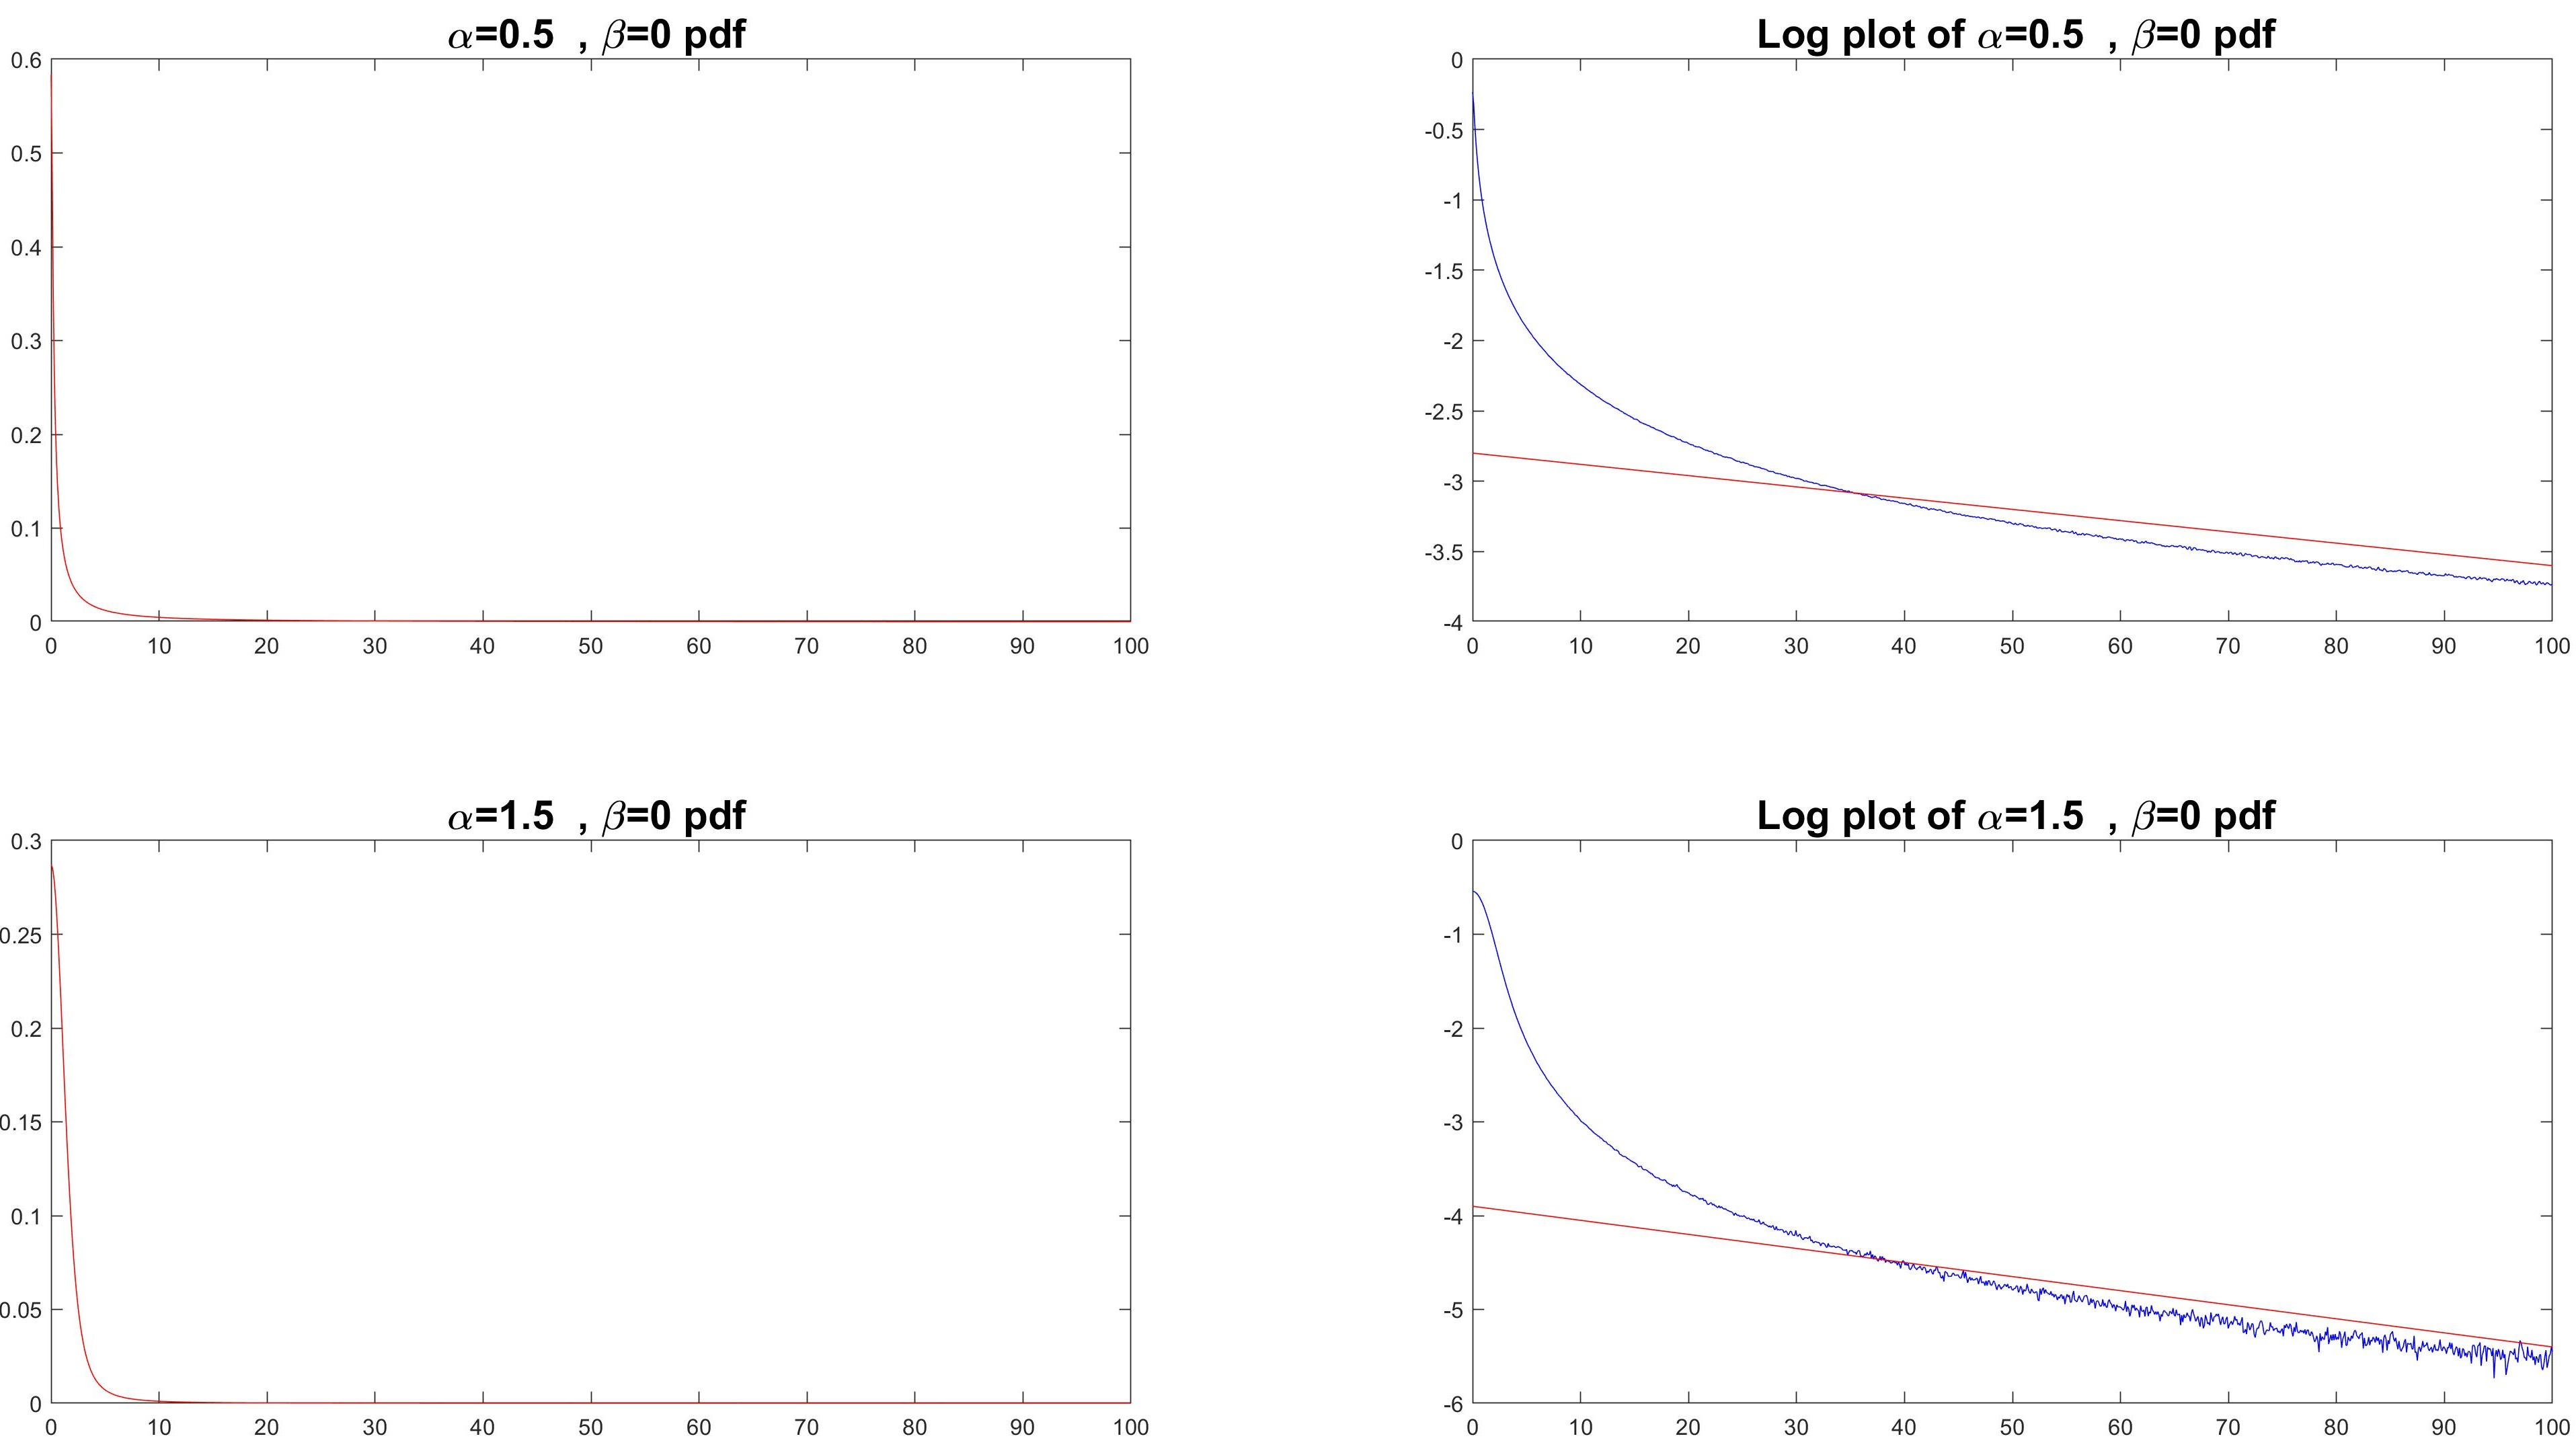
\includegraphics[width=\linewidth]{4ftr1}
  \caption{Pdf and log(pdf)of the distribution with $\beta = 0 $ and $ \alpha =0.5 , 1.5$}
  \label{fig:4ftr1}
\end{figure}

\begin{figure}[h]
  \centering
    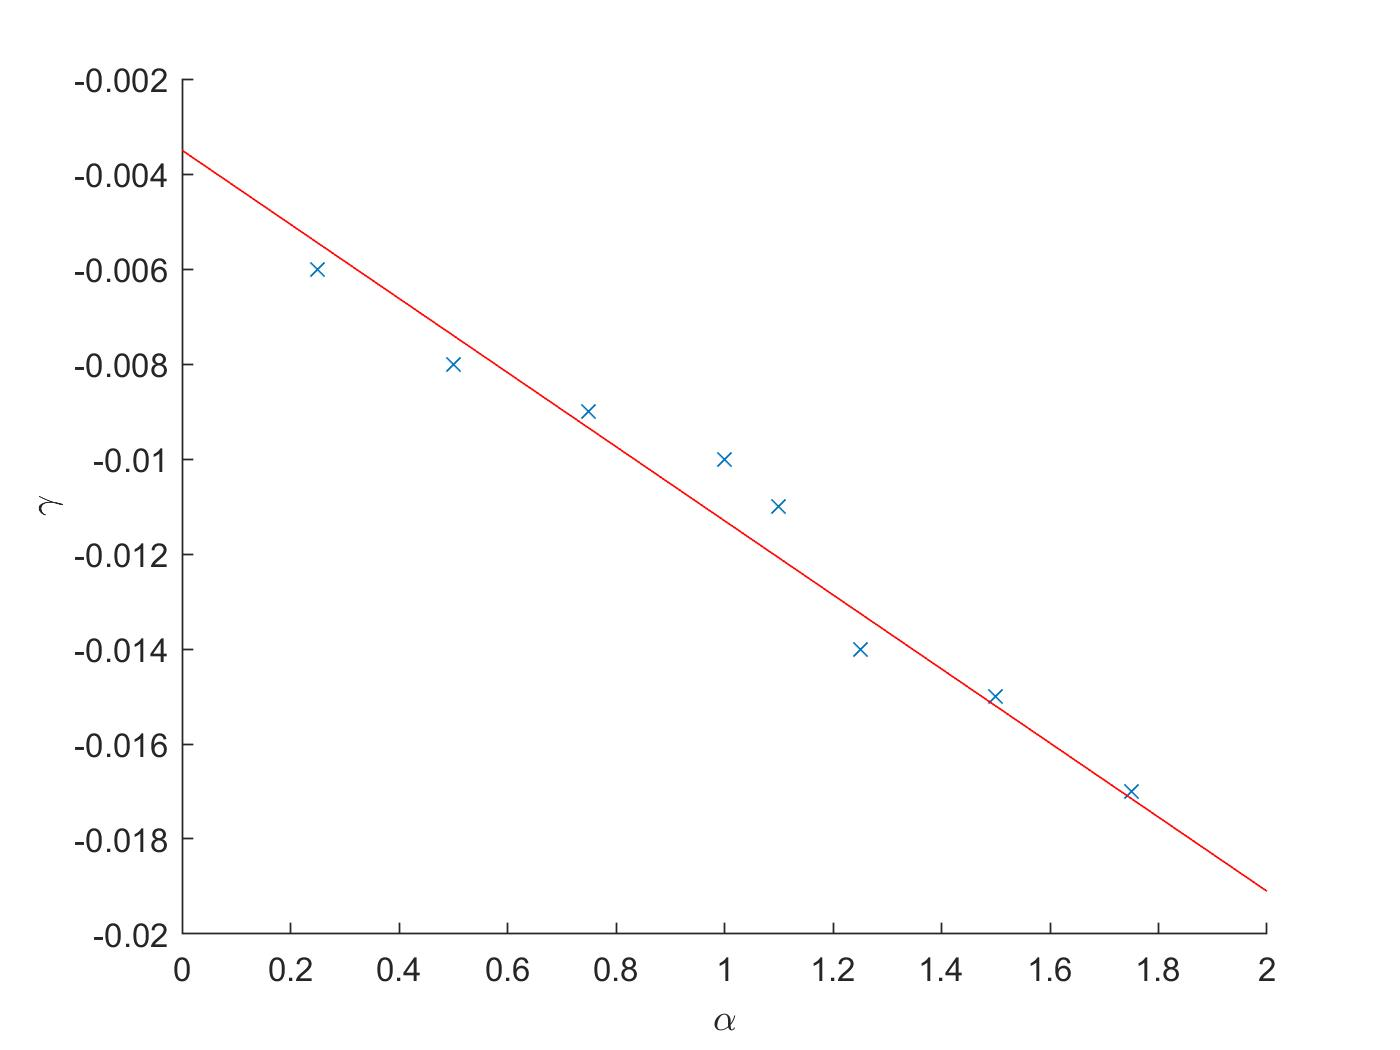
\includegraphics[width=\linewidth]{4ftr2}
  \caption{Relationship between $\alpha$ and $\gamma$ at large x values. $\gamma=-0.0078\alpha-0.0035$}
  \label{fig:4ftr2}
\end{figure}

The tail behaviour of the pdf p(x) can be approximated to a curve $cx^\gamma$ at large x values. In order to work out this relationship a log plot can be constructed of the pdf. The pdf is calculated using a kernel smoothing technique of the random vector X. A large sample size is required to accurately get this relationship as p(x) at x=100 is approximately $10^{-4}$ and $5x10^{-6}$ for alpha = 0.5 and 1.5. This means in order to get sufficient random variables in this region sample size has to be large. A sample size of 100 million was used. The pdf and log plots can be seen in figure \ref{fig:4ftr1}. From these plots  $\gamma$ is the gradient at large x on the log plot, it was found to be -0.008 and -0.015 for alpha = 0.5 and 1.5 respectively. LogC varied across repeats but was in the range -2.8 and -3.8 for the two distributions. In order to see how $\gamma$ is related to $\alpha$ distributions with other $alpha$ values were tested, these are plotted in \ref{fig:4ftr2}. The linear relationship $\gamma=-0.0078\alpha-0.0035$ was calculated.

\subsubsection{Links with the Gaussian}

By plotting the pdf of the distribution for various $\alpha$ values as shown in figure \ref{fig:4ftr3} links between the Gaussian can be found. When $\alpha$ approaches 2 it closely matches and eventually is a Gaussian distribution $\mathcal{N}(0,2)$. 

\subsubsection{Matlab code} %-------------------------
The Matlab code for this transformation can be seen in sections 4.0 - 4.3 of the appendix.

\section{Conclusion}
%---------------------------------------------------
Through the investigations carried out through this lab it has become clear that Matlab random number generation follows the theory such as the multinomial distribution. Through the use of transformations either directly or using inverse CDF complicated distributions can be generated from much simpler ones such as uniform and Gaussian. Sample size decreased spread throughout the experiments producing smoother curves, histograms and better estimators. The alpha stable distribution is an example of a difficult density that can be generated using these methods. This distribution tends to a Gaussian as $\alpha$ tends to 2 and skewness is created by the $\beta$ variable. This distribution can be expressed in the form $cx^{\gamma}$ for large x. The sample mean of distributions can be estimated using a Monte Carlo approach which produced an unbiased estimator with accuracy increasing with $1/\sqrt{N}$. Transforming distributions proves very useful in real word applications as it means lots of desired distributions can be generated from the same technology that for reliably produces a uniform distribution.
%------------------------------------------------

\section{Appendix}
\begin{large}
1.0 Uniform and normal random variables
\end{large}
\newline
\begin{itshape}
\%Plot Normal Distributions\\
figure(1)\\
x=randn(1000,1);\\
subplot(211),\\
histogram(x,20)\\
hold on\\
n = [-3:.1:3];\\
norm = normpdf(n,0,1)*350;\\
plot(n,norm,'red')\\
hold off\\
subplot(212),\\
ksdensity(x,'width',0.1)\\
hold on\\
n = [-3:.1:3];\\
norm = normpdf(n,0,1);\\
plot(n,norm,'red')\\
hold off\\

\%plot Uniform Distribution\\
figure(2)\\
y=rand(1000,1);\\
subplot(211),\\
histogram(y,10)\\
axis([0 1 0 150])\\
hold on\\
height = 100.* ones(length(n),1)\\
plot(n,height,'red')\\
hold off\\
subplot(212),\\
ksdensity(y,'width',0.1)\\
hold on\\
x1=[0,0,1,1];\\
y1=[0,1,1,0];\\
plot(x1,y1,'red')\\
hold off\\

\%plot Uniform no.2 Distribution\\
N=[100,1000,10000]\\
height=[20,150,1200]\\
figure(3)\\
for i =1:3 \\
	y=rand(N(i),1);\\
	subplot(3,1,i),\\
	histogram(y,10)\\
	title(['N=',num2str(N(i))])\\
	hold on\\
	mean=N(i)*0.1;\\
	sd= sqrt(N(i)*0.1*0.9);\\
	line([0,1],[mean,mean],'color','red')\\
	line([0,1],[mean+3*sd,mean+3*sd],'color','red')\\
	line([0,1],[mean-3*sd,mean-3*sd],'color','red')\\
	axis([0 1 0 height(i)])\\
	hold off\\
end\\
\end{itshape}

\begin{large}
1.1 Gaussian bin probabilities
\end{large}
\newline
\begin{itshape}

\%plot Normal distribution  Distribution\\
N=[100,1000,10000]\\
height=[20,150,1200]\\
figure(1)\\

for i =1:3 \\
botrange=0;\\
y=randn(N(i),1);\\
subplot(3,1,i),\\
numberofbins = 21;\\
binranges = zeros(numberofbins,1);\\
for j = 1:numberofbins+1\\
    binranges(j) = (3--3)/(numberofbins-1) *(j-1) + -3.15;\\
end\\
histogram(y,binranges)\\
hold on\\
for j = 1:length(binranges)-1\\
    pj = normcdf(binranges(j+1)) - normcdf(binranges(j));\\
    mean = N(i)*pj;\\
    sd = sqrt(N(i)*pj*(1-pj))*3;\\
    if j==length(binranges)/2\\
        toprange = (mean + sd )*1.1;\\
    end\\
    tempbot= (mean-sd)*1.1;\\
    if tempbot <botrange\\
        botrange=tempbot;\\
    end\\
    line([binranges(j),binranges(j+1)],  [mean,mean],'color','red', 'LineWidth',1)\\
     line([binranges(j),binranges(j+1)],[mean+sd,mean+sd],
     'color',[0 0.5 0],'LineWidth',1)\\
    line([binranges(j),binranges(j+1)],[mean-sd,mean-sd],
    'color',[0 0.5 0],'LineWidth',1)\\
end\\
hold off  \\
axis([-3.5 3.5 botrange toprange])\\
title(['N=',num2str(N(i))])\\
end\\
\end{itshape}


\begin{large}
2.0 Transforming a Gaussian by Y=aX+b
\end{large}
\newline
\begin{itshape}
x=randn(1000,1);\\
a=2;\\
b=1;\\
y=a*x+b;\\
J=abs(a);\\

py=0;\\
for i = 1:1 \%only one possible value for x given y\\
    py = normpdf((y-b)/a,0,1)/J ;\\
end\\
    
\%Plot Transformed Distributions\\
figure(1)\\
subplot(221),\\
histogram(y,20)\\
hold on\\
scatter(y,py*700,'blue')\\
f = @(x) 1/(sqrt(2*pi)*a) *exp(-0.5*(x-b)\^{} 2/(a\^{} 2)) *700\\
fplot(f,[-5,5],'red','LineWidth',1.5)\\
hold off\\
title('\textbackslash fontsize\{14\} a=2, b=1')\\

subplot(222),\\
a=10;\\
b=1;\\
y=a*x+b;\\
J=abs(a);\\
py=0;\\
for i = 1:1 \%only one possible value for x given y\\
    py = normpdf((y-b)/a,0,1)/J ;\\
end\\
histogram(y,20)\\
hold on\\
scatter(y,py*3200,'blue')\\
f = @(x) 1/(sqrt(2*pi)*a) *exp(-0.5*(x-b)\^{}2/(a\^{}2)) *3200\\
fplot(f,[-25,25],'red','LineWidth',1.5)\\
hold off\\
title('\textbackslash fontsize\{14\} a=10, b=1')\\

subplot(223),\\
a=2;\\
b=10;\\
y=a*x+b;\\
J=abs(a);\\
py=0;\\
for i = 1:1 \%only one possible value for x given y\\
    py = normpdf((y-b)/a,0,1)/J ;\\
end\\
histogram(y,20)\\
hold on\\
scatter(y,py*700,'blue')\\
f = @(x) 1/(sqrt(2*pi)*a) *exp(-0.5*(x-b)\^{}2/(a\^{}2)) *700\\
fplot(f,[5,15],'red','LineWidth',1.5)\\
hold off\\
title('\textbackslash fontsize\{14\} a=2, b=10')\\

subplot(224),\\
a=10;\\
b=10;\\
y=a*x+b;\\
J=abs(a);\\
py=0;\\
for i = 1:1 \%only one possible value for x given y\\
    py = normpdf((y-b)/a,0,1)/J ;\\
end\\
histogram(y,20)\\
hold on\\
scatter(y,py*3200,'blue')\\
f = @(x) 1/(sqrt(2*pi)*a) *exp(-0.5*(x-b)\^{}2/(a\^{}2)) *3200\\
fplot(f,[-25,40],'red','LineWidth',1.5)\\
hold off\\
title('\textbackslash fontsize{14} a=10, b=10')\\

\end{itshape}

\begin{large}
2.1 Transforming a Gaussian by $Y=X^2$
\end{large}
\newline
\begin{itshape}
x=randn(1000,1);\\
y=x.\^{}2;   \\
py=zeros(length(y),1);\\
for i = 1:2 \%y=x\^{}2 is a 2:1 function\\
    J=abs(x)*2;\\
    py = py + normpdf((-1)\^{}i*sqrt(y),0,1)./J ;\\
end\\

\%Plot Transformed distribution\\
figure(1)\\
histogram(y,40)\\
hold on\\
scatter(y,py*400,'blue')\\
f = @(x) 1/(sqrt(2*pi*x)) *exp(-0.5*(sqrt(x))\^{}2) *400\\
fplot(f,[0,7],'red','LineWidth',1.5)\\
hold off\\
title('y=x\^{}2')\\
axis([0 10 0 750])\\
\end{itshape}


\begin{large}
2.2 Transforming a Gaussian by $y=sin(x)$ and $y=min[sin(x),x]$
\end{large}
\newline
\begin{itshape}
x=rand(1000,1)*2*pi; \%uniform distribution\\
y=sin(x);\\
figure(2)\\
yclip=min(y,0.7);\\
scatter(yclip,x)\\
xlabel('y')\\
ylabel('x')\\
py=zeros(length(y),1);\\
for i = 1:1 \%y=sin(x) is a 1:1 function in range 0-2pi  \\
    J=abs(cos(x));\\
    py = py + (1/(2*pi))./J ; \% as p(x) = 1/2pi everywhere \\
end\\

binrange=[0,0.05,0.1,0.15,0.2,0.25,0.3,0.35,0.4,0.45, 0.5,0.55,0.6,0.65,0.7,0.75,0.8,0.85,0.9,0.95,1]\\
\%Plot Transformed distribution\\
figure(1)\\
subplot(211)\\
histogram(y,binrange)\\
hold on\\
scatter(y,py*150,'blue')\\
f = @(x) 1/(2*pi*abs(cos(asin(x)))) *150;\\ 
fplot(f,[0,1],'red','LineWidth',1.5)\\
hold off\\
title('y=sin(x)')\\
axis([0 1 0 150])\\
binrange=[0,0.05,0.1,0.15,0.2,0.25,0.3,0.35,0.4,0.45, 0.5,0.55,0.6,0.65,0.69,0.71] \% in order to see peak at 0.7\\
subplot(212)\\
histogram(yclip,binrange)\\
hold on\\
f = @(x) 1/(2*pi*abs(cos(asin(x)))) *150; \\
fplot(f,[0,0.7],'red','LineWidth',1.5)\\
top=1/(2*pi)*(pi-2*asin(0.7))*1000 \% times 1000 as its a p(y)*N = number in histogram here\\
line([0.7 0.7],[0 top],'color', 'red', 'LineWidth',1.5)\\
hold off\\
title('y=sin(x) clippied at y=0.7')\\
axis([0 1 0 350])\\
\end{itshape}

\begin{large}
3.0 Generating an exponential distribution using CDF method
\end{large}
\newline
\begin{itshape}
x=rand(1000,1);\\
y= -log(-x+1);\\

figure(1)\\
subplot(211),\\
histogram(y,20);\\
hold on \\
f = @(x) 400*exp(-x)\\
fplot(f,[0,7],'red')\\
hold off\\
subplot(212),\\
ksdensity(y,'width',0.1)\\
hold on \\
f = @(x) exp(-x)\\
fplot(f,[0,7],'red')\\
hold off\\
\end{itshape}


\begin{large}
3.0 Generating an exponential distribution using CDF method
\end{large}
\newline
\begin{itshape}
M=100;\\
x=rand(M,1);\\
y=-log(-x+1);\\
\\
N=3;\\
mean = zeros(M,1);\\
variance = zeros(M,1);\\
meansquarederror = zeros(M,N);\\
mse=zeros(M,1);\\
vse=zeros(M,1);\\
variancesquarederror = zeros(M,N);\\
range=zeros(M,1);\\

for j =1:N\\
xs=rand(M,M);\\
f = @(x) -log(-x+1);\\
ys= arrayfun(f,xs);\\
for i = 1:M\\
    mean(i)=sum(ys(i,:))/M;\\
    variance(i)=sum(ys(i,:).*ys(i,:))/M - mean(i)*mean(i);\\
    temp= sum(ys(i,1:i))/i;\\
    meansquarederror(i,j)= temp;\\
    variancesquarederror(i,j)= sum(ys(i,1:i).*ys(i,1:i))/i - temp*temp;\\
    range(i)=i;\\
end
samplegroupmean=sum(mean)/M;\\
samplegroupvariance=sum(variance.*variance)/M;\\
end\\
for i = 1:M\\
   mse(i)=sum(meansquarederror(i,:))/N; \\
   vse(i)=sum(variancesquarederror(i,:))/N;\\
end\\
figure(2)\\
subplot(211)\\
plot(range,(mse-1).*(mse-1)*5);\\
f = @(x) 1/(x);\\
hold on\\
fplot(f,[0,M],'red')\\
hold off\\
axis([0 100 0 0.5])\\
title('Mean Squared Error')\\
xlabel('Sample Size')\\
ylabel('Error Squared')\\
subplot(212)\\
plot(range,(vse-1).*(vse-1));\\
f = @(x) 1/(2*sqrt(x));\\
hold on\\
fplot(f,[0,M],'red')\\
hold off\\
axis([0 100 0 1])\\
title('Variance Squared Error')\\
xlabel('Sample Size')\\
ylabel('Error Squared')\\
\end{itshape}



\begin{large}
4.0 Simulation from a difficult density
\end{large}
\newline
\begin{itshape}
v=exprnd(1,1000,1);\\
u=rand(1000,1);\\
u=(u-0.5)*pi ;\\
alpha=0.5;\\
betavals=[-1,-0.5,0,0.5,1,-1,-0.5,0,0.5,1];\\
x=zeros(length(u),10);\\

figure(1)\\
histrange=50;\\
range=700;\\

for i = 1:10\\
beta = betavals(i);\\
if i>5\\
    alpha = 1.5;\\
    histrange=10;\\
    range=400;\\
end \\
b=1/alpha * atan(beta*tan(pi*alpha/2)) ;\\
s=(1+beta\^{}2*(tan(pi*alpha/2))\^{}2)\^{}(1/(2*alpha));\\
x(:,i)=s* sin(alpha*(u+b))./(cos(u).\^{}(1/alpha)).* (cos(u-alpha*(u+b))./v).\^{}((1-alpha)/alpha); \\
subplot(2,5,i),\\
histogram(x(:,i),[-histrange:histrange/10:histrange])\\
axis([-histrange histrange 0 range])\\
tit = strcat('\textbackslash fontsize\{18\} \textbackslash alpha=',num2str(alpha), '\textbackslash fontsize\{18\} , \textbackslash beta=',num2str(beta));\\
title(tit)\\
end\\
\end{itshape}



\begin{large}
4.1 Tail probabilities
\end{large}
\newline
\begin{itshape}
v=exprnd(1,10000,1);\\
u=rand(10000,1);\\
u=(u-0.5)*pi ;\\
alphavals=[0.5,1.5];\\
beta=0;\\
tvalues=[0,1,3,6];\\
x=zeros(length(u),2);\\
tailprob=zeros(4,4);\\

for i = 1:2\\
alpha = alphavals(i);\\
b=1/alpha * atan(beta*tan(pi*alpha/2)) ;\\
s=(1+beta\^{}2*(tan(pi*alpha/2))\^{}2)\^{}(1/(2*alpha));\\
x(:,i)=s* sin(alpha*(u+b))./(cos(u).\^{}(1/alpha)).* (cos(u-alpha*(u+b))./v).\^{}((1-alpha)/alpha); \\
for j = 1:length(u) \%calculate tail probabilities\\
   X=abs(x(j,i));\\
   if X > tvalues(4)\\
       tailprob(:,i)=tailprob(:,i)+1;\\
   elseif X>tvalues(3)\\
       tailprob(1:3,i)=tailprob(1:3,i)+1;\\
   elseif X>tvalues(2)\\
       tailprob(1:2,i)=tailprob(1:2,i)+1;\\
   elseif X>tvalues(1)\\
       tailprob(1,i)=tailprob(1,i)+1;\\
   end       \\
end\\
end\\
tailprob=tailprob./length(u);\\
for i = 1:length(tvalues)\\
   tailprob(i,3:4)=2*normcdf(-tvalues(i)); \\
end\\
tailprob\\

figure(1)\\

subplot(2,1,1),\\
histogram(x(:,1),[-10:10/20:10])\\
axis([-10 10 0 2000])\\
tit = strcat('\textbackslash fontsize\{18\} \textbackslash alpha=0.5 \textbackslash fontsize\{18\} , \textbackslash beta=0');\\
title(tit)\\
hold on\\
n = [-10:.1:10];\\
norm = 4000*normpdf(n,0,1);\\
plot(n,norm,'red')\\
hold off\\

subplot(2,1,2),\\
histogram(x(:,2),[-10:10/20:10])\\
axis([-10 10 0 2000])\\
tit = strcat('\textbackslash fontsize\{18\} \textbackslash alpha=1.5 \textbackslash fontsize\{18\} , \textbackslash beta=0');\\
title(tit)\\
hold on\\
n = [-10:.1:10];\\
norm = 3000*normpdf(n,0,1);\\
plot(n,norm,'red')\\
hold off\\
\end{itshape}



\begin{large}
4.2 Calculating gamma
\end{large}
\newline
\begin{itshape}
v=exprnd(1,10000000,1);\\
u=rand(10000000,1);\\
u=(u-0.5)*pi ;\\
alphavals=[0.5,1.5];\\
beta=0;\\
x=zeros(length(u),2);\\
pdfx=zeros(1000,2);\\
xi=zeros(1000,2);\\
pts = linspace(0,100,1000); \% points to evaluate the estimator\\
for i = 1:2\\
alpha = alphavals(i);\\
b=1/alpha * atan(beta*tan(pi*alpha/2)) ;\\
s=(1+beta\^{}2*(tan(pi*alpha/2))\^{}2)\^{}(1/(2*alpha));\\
x(:,i)=s* sin(alpha*(u+b))./(cos(u).\^{}(1/alpha)).* (cos(u-alpha*(u+b))./v).\^{}((1-alpha)/alpha);\\ 
(p,xd]=ksdensity(x(:,i),pts);\\
pdfx(:,i)=p;\\
xi(:,i)=xd;\\
end\\
figure(1)\\
lgpdfx=log10(pdfx);\\
subplot(2,2,1),\\
plot(xi(:,1),pdfx(:,1),'red')\\
tit = strcat('\textbackslash fontsize\{18\} \textbackslash alpha=0.5 \textbackslash fontsize\{18\} , \textbackslash beta=0 pdf');\\
title(tit)\\
subplot(2,2,2)\\
plot(xi(:,1),lgpdfx(:,1),'blue')\\
tit = strcat('\textbackslash fontsize\{18\}Log plot of \textbackslash alpha=0.5 \textbackslash fontsize\{18\} , \textbackslash beta=0 pdf');\\
title(tit)\\
xlim([0 100]);\\
f = @(x) -0.008*x-2.8;\\
hold on\\
fplot(f,[0,100],'red')\\
hold off\\


subplot(2,2,3),\\
plot(xi(:,2),pdfx(:,2),'red')\\
%axis([-20 20 0 1])\\
tit = strcat('\textbackslash fontsize\{18\} \textbackslash alpha=1.5 \textbackslash fontsize\{18\} , \textbackslash beta=0 pdf');\\
title(tit)\\
subplot(2,2,4)\\
plot(xi(:,2),lgpdfx(:,2),'blue')\\
tit = strcat(' \textbackslash fontsize\{18\}Log plot of \textbackslash alpha=1.5 \textbackslash fontsize\{18\} , \textbackslash beta=0 pdf');\\
title(tit)\\
xlim([0 100]);\\
f = @(x) -0.015*x-3.9;\\
hold on\\
fplot(f,[0,100],'red')\\
hold off\\
\end{itshape}

\begin{large}
4.3 Links to the Gaussian
\end{large}
\newline
\begin{itshape}
v=exprnd(1,1000000,1);\\
u=rand(1000000,1);\\
u=(u-0.5)*pi ;\\
alphavals=[0.5,1,1.5,1.75,2];\\
beta=0;\\
x=zeros(length(u),length(alphavals));\\
pdfx=zeros(1000,length(alphavals));\\
xi=zeros(1000,length(alphavals));\\
pts = linspace(-4,4,1000); \% points to evaluate the estimator\\
for i = 1:length(alphavals)\\
alpha = alphavals(i);\\
b=1/alpha * atan(beta*tan(pi*alpha/2)) ;\\
s=(1+beta\^{}2*(tan(pi*alpha/2))\^{}2)\^{}(1/(2*alpha));\\
x(:,i)=s* sin(alpha*(u+b))./(cos(u).\^{}(1/alpha)).* (cos(u-alpha*(u+b))./v).\^{}((1-alpha)/alpha); \\
(p,xd]=ksdensity(x(:,i),pts);\\
pdfx(:,i)=p;\\
xi(:,i)=xd;\\
end\\
figure(1)\\
n = [-4:.1:4];\\
for i = 1:length(alphavals)\\
   hold on\\
   plot(xi(:,i),pdfx(:,i),'LineWidth',1)\\
   hold off\\
end\\
hold on\\
norm = normpdf(n,0,sqrt(2));\\
plot(n,norm,'--red','LineWidth',1)\\
hold off\\
legend('\textbackslash alpha = 0.5','\textbackslash alpha = 1','\textbackslash alpha = 1.5','\textbackslash alpha = 1.75','\textbackslash alpha = 2','Gaussian(0,2)')\\
\end{itshape}


%------------------------------------------------
\end{document}
